\documentclass{article}
\usepackage[english]{babel}
\usepackage[utf8]{inputenc}
\usepackage{vmargin}
\usepackage{amssymb}
\usepackage{amsmath}
\usepackage{graphicx}
\usepackage{caption}
\usepackage{subcaption}
\usepackage{url}
\usepackage[font=itshape]{quoting}
\usepackage[T1]{fontenc} 
\usepackage[sorting=none]{biblatex}
\usepackage{csquotes}
\usepackage{float}
\addbibresource{biblio.bib}

\setmarginsrb{2 cm}{2 cm}{2 cm}{2 cm} {1.1 cm}{1.1 cm}{1 cm}{1.5 cm}

\title{MULTIVARIABLE CONTROL AND
COORDINATION SYSTEMS
(EE-477)
}
\author{Baptiste Savioz }
\date{January 2022}

\setcounter{MaxMatrixCols}{20}
\begin{document}


\label{page:titre}
\begin{titlepage}
    \begin{center}
        %\vspace*{1cm}

        \Huge
        \textbf{Path tracking for an automated vehicle}\\
        \vspace{0.3cm}
        Case study report
        \vspace{0.5cm}
        \LARGE
        
            
        \vspace{1.5cm}

        \textbf{Baptiste Savioz 284253}\\

        \vfill
            
            
        \vspace{0.8cm}
        
        %\includegraphics[width=0.4\textwidth]{images/SSB.png}
        
\includegraphics[width=0.4\textwidth]{Latex report/image/epfl.png}
        
        \Large
        Multivariable control and coordination systems (EE-477)\\
        Prof. Gillet Denis\\
        EPFL\\
        Fall 2022
            
    \end{center}
\end{titlepage}

\newpage
\tableofcontents
\newpage


\section{Modeling, linearization, and discretization}
\label{sec:modeling}
\subsection{Problem definition}
\subsubsection*{System's variable}
\begin{itemize}
    \item Reference path $\pi$, $\pi : \mathbb{R} \longrightarrow \mathbb{R}^3, \quad \pi(s_\pi) = (x_\pi, y_\pi,\theta_\pi)$
    \item Distance $s$ : $s \in \mathbb{R}$, distance along the path corresponding to the vehicle’s position projections.
    \item Lateral error $d$ : $d \in \mathbb{R},\quad d = ||P_r - P_{r,\pi}||$, distance between the path and the vehicle.
    \item heading error $s$ : $\theta_e \in \mathbb{R}, \quad \theta_e = (\theta - \theta_\pi)$, difference between vehicle yaw angle and path's orientation.
    \item Longitudinal speed $v$ : $v \in \mathbb{R}^+$
    \item Longitudinal speed reference $v_{ref}$ : $v_{ref} \in \mathbb{R}^+$
    \item Steering wheel position $\phi$ : $\phi \in \mathbb{R}$
    \item Steering wheel reference $\phi_{ref}$ : $\phi_{ref} \in [-4\pi,4\pi]$
    \item Path's curvature $\kappa$
\end{itemize}

\begin{figure}[H]
    \centering
    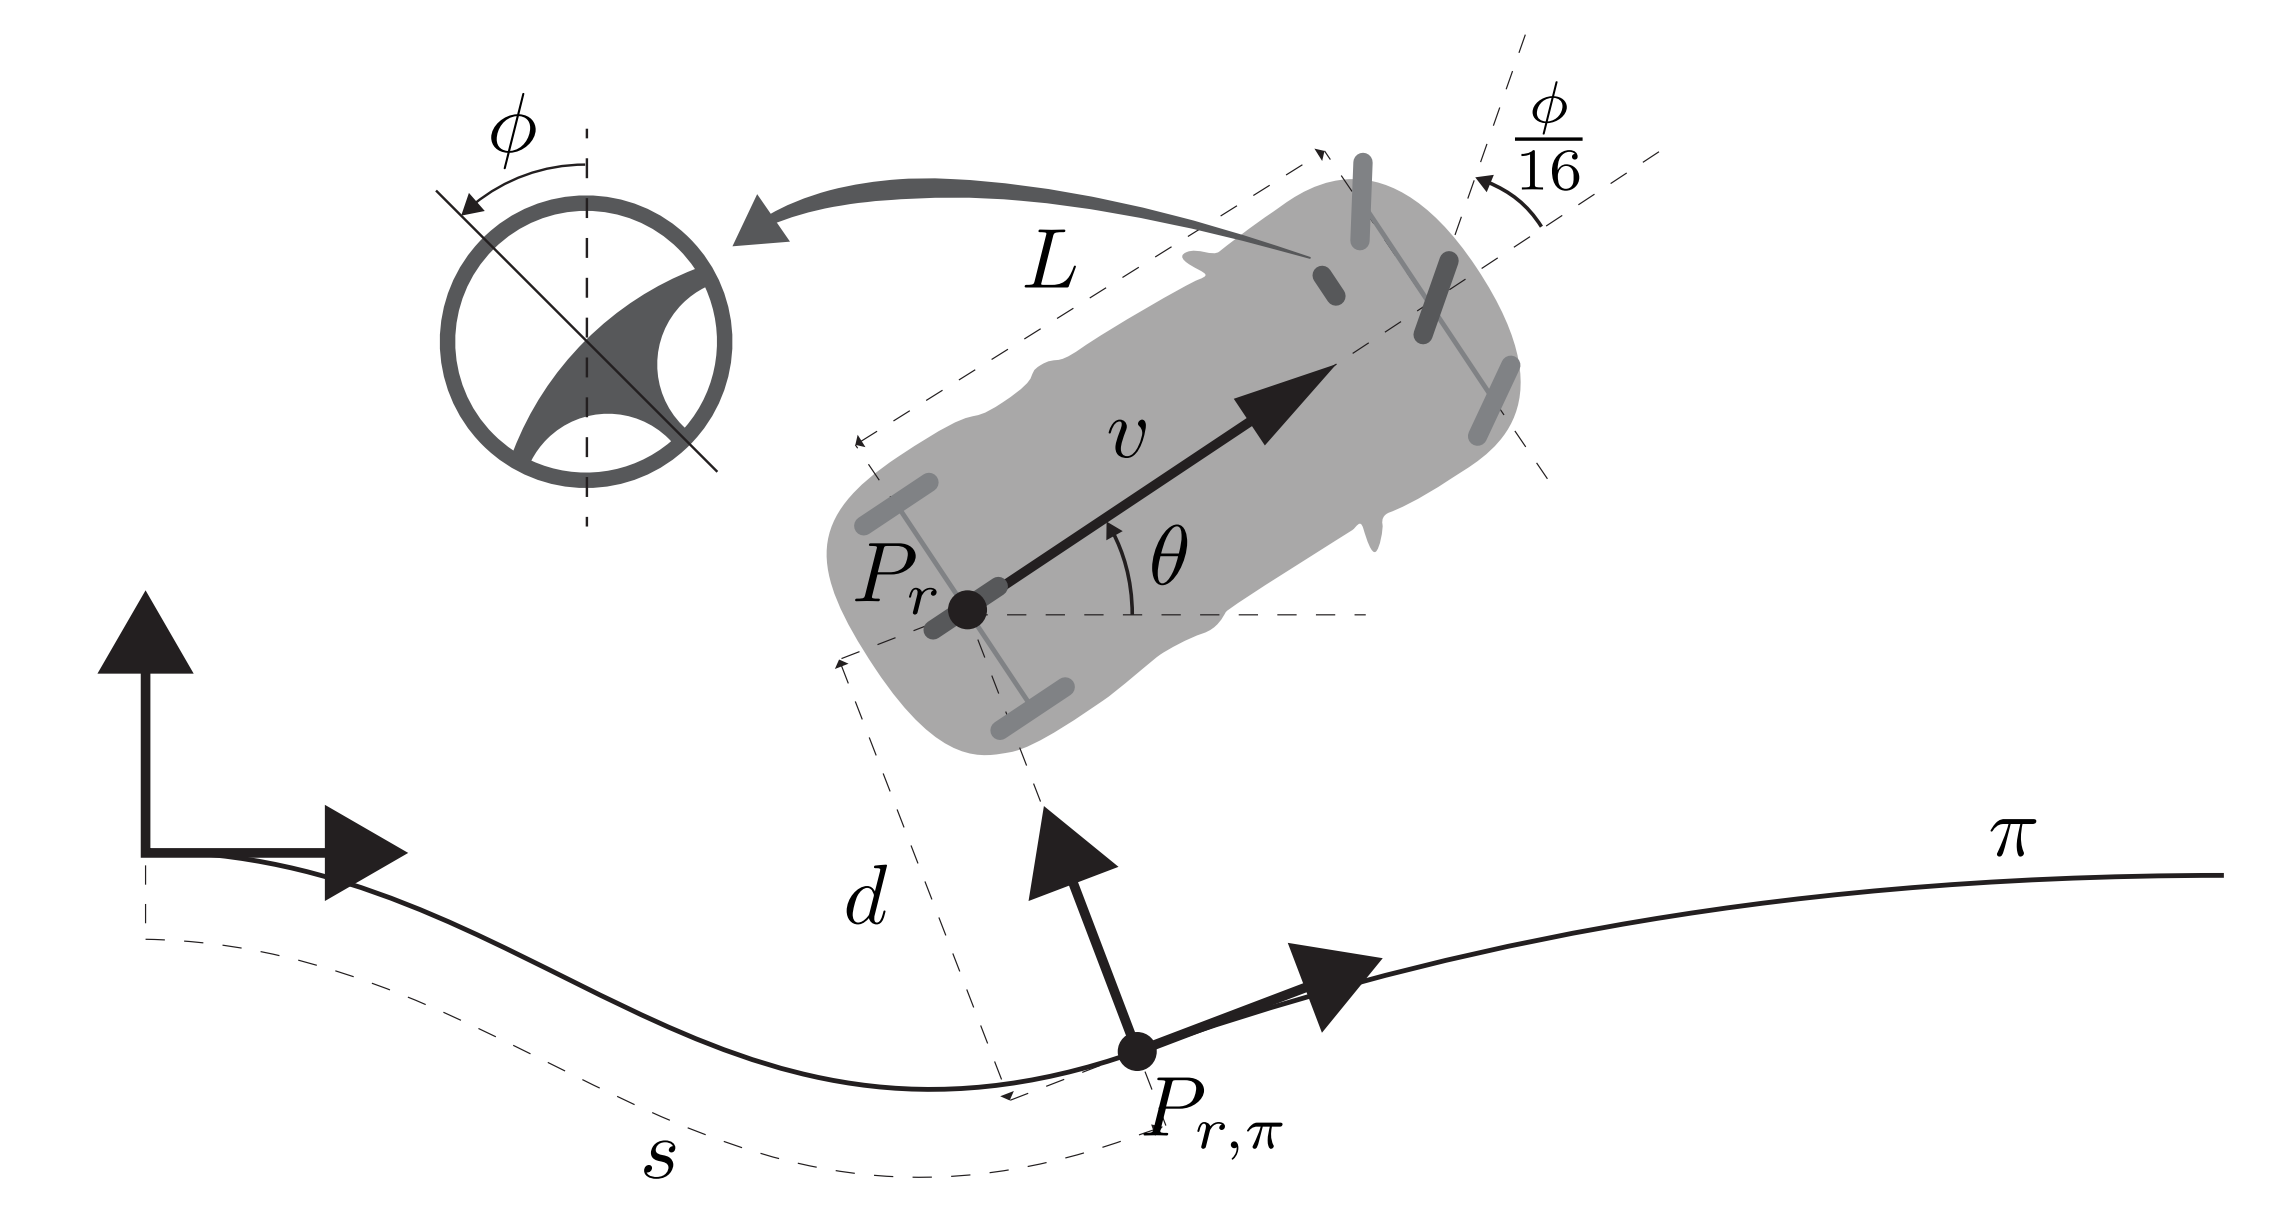
\includegraphics[width=0.6\textwidth]{Latex report/image/system_def.png}
    \caption{Coordinate system}
    \label{fig:sys_def}
\end{figure}

\subsubsection*{System's model}
With the variable defined above, one may write the dynamic of the system with the following equations :
\begin{align}
    \dot{s} &= \frac{v \cos(\theta_e)}{1 - d\kappa(s)}\\
    \dot{d} &= v \sin(\theta_e)\\
    \dot{\theta_e} &= \frac{v}{L}\tan(\frac{\phi}{16}) - \kappa(s)\dot{s}\\
    \dot{v} &= \sigma_v (v_{ref} - v)\\
    \dot{\phi} &= \sigma_{ref} (\phi_{ref} - \phi)\\
\end{align}
\\
In the following, state measurement is assumed unless stated otherwise and the states and control input of the system are :
\begin{align}
    \bold{x} &= [x_1, x_2, x_3, x_4, x_5] = [s,d,\theta_e, v, \phi]\\
    \bold{u} &= [u_1, u_2] = [v_{ref}, \phi_{ref}]\\
    \bold{y} &= \bold{x}
\end{align}


\subsection{Questions}
\subsubsection*{Question 0.1 : Rewrite the non-linear model in the standart form $\bold{\dot{x}} = f(\bold{x}, \bold{u})$}
\begin{equation}
    \left[ {\begin{array}{c}
        \dot{x}_1\\
        \dot{x}_2\\
        \dot{x}_3\\
        \dot{x}_4\\
        \dot{x}_5\\
    \end{array} } \right]
    =
    \left[ {\begin{array}{c}
        f_1(x)\\
        f_2(x)\\
        f_3(x)\\
        f_4(x)\\
        f_5(x)\\
    \end{array} } \right] 
    =
    \left[ {\begin{array}{c}
        \frac{x_4 \cos(x_3)}{1 - x_2\kappa(x_1)}\\
        x_4 \sin(x_3)\\
        \frac{x_4}{L}\tan(\frac{x_5}{16}) - \frac{\kappa(x_1) x_4 \cos(x_3)}{1 - x_2 \kappa(x_1)}\\
        \sigma_v (u_1 - x_4)\\
        \sigma_{ref} (u_2 - x_5)\\
    \end{array} } \right]
\end{equation}



\subsubsection*{Question 0.2 : Given the chosen state space, why it wouldn’t be appropriate linearizing the system around a nominal point.}
There are no such point that are good around the whole trajectory.



\subsubsection*{Question 0.3 : Calculate the nominal trajectory representing the constant-speed perfect tracking situation (that is, a situation where the vehicle drives perfectly on the path and at a constant speed $\bold{v_{ref}}$ ) for a path of constant curvature $\bold{\kappa_{ref}}$.}
Several assumption are made that implies the following :
\begin{itemize}
    \item Constant path curvature : $\kappa(s) \longrightarrow \kappa_{ref}$
    \item Constant speed : $v(s) \longrightarrow v_{ref}$
    \item Vehicle drives perfectly on the the path $\longrightarrow$ no error and no error dynamics ($d=0, \dot{d}=0, \theta_e=0, \dot{\theta_e}=0$)
\end{itemize}
Thus, we already know $\bar{x}_2(t) = 0$, $\bar{x}_3(t) = 0$, $\bar{x}_4 = u_1$. In order to find $\Bar{x}_1(t)$, one can substitute the known variable in $f_1(x)$

\begin{equation}\begin{align}
    \dot{\Bar{x}}_1(t) =  \frac{\bar{x}_4 \cos(\bar{x}_3)}{1 - \bar{x}_2\kappa(s)}
        =v_{ref} = u_1  
\end{align} \end{equation}
By integration, one may find :
\begin{equation}
    \Bar{x}_1(t) = u_1 t + s_0
\end{equation}
\\
Moreover, to find $\bar{x}_5(t)$,  one may want to use $f_3(t)$ and substitute with the known variable.
\begin{equation}\begin{align}
    \dot{\bar{x}}_3 &= f_3(\bar{x}) =
    \frac{\bar{x}_4}{L}\tan\left(\frac{\bar{x}_5}{16}\right) - \frac{\kappa(\bar{x}_1) \bar{x}_4 \cos(\bar{x}_3)}{1 - x_2 \kappa(\bar{x}_1)} \iff\\
    0 &= \frac{v_{ref}}{L}\tan\left(\frac{\bar{x}_5}{16}\right) - \kappa_{ref}v_{ref} \iff\\
    \bar{x}_5 &= 16\tan^{-1}\left(\kappa_{ref}L\right)
\end{align}\end{equation}
\\
 Finally, one can write the nominal trajectory as :
\begin{equation}
    \bar{x}
    =
    \left[ {\begin{array}{c}
        \bar{x}_1(t)\\
        \bar{x}_2(t)\\
        \bar{x}_3(t)\\
        \bar{x}_4(t)\\
        \bar{x}_5(t)\\
    \end{array} } \right]
    =
    \left[ {\begin{array}{c}
        u_1 t + s_0\\
        0\\
        0\\
        u_1\\
        16 \tan^{-1}(\kappa_{ref} L)\\
    \end{array} } \right]
    \label{eq:trajectory}
\end{equation}



\subsubsection*{Question 0.4 : Linearize the system around such a nominal trajectory.}
In this part, we will introduce the linearized model of the system. The linearization is done around a point, or in our case, around a trajectory (equation \ref{eq:trajectory}) and for this purpose, we will introduce the small signal linearization, which is the deviation of the state from an nominal point/trajectory.\\
\\
Small signal linerization :
\begin{equation}
    \begin{align}
        \Tilde{x} &= x - \Bar{x}\\
        \Tilde{y} &= y - \Bar{y}\\
        \Tilde{u} &= u - \Bar{u}  
    \end{align}
\end{equation}

Starting from there, the first step is to find the matrices $A$ and $B$ of the linear system using the first order Taylor expansion of the non-linear model.
\begin{align}
    A &= 
    \left[ {\begin{array}{cccc}
        \frac{\partial f_1}{\partial x_1} & \frac{\partial f_1}{\partial x_2} & \cdots & \frac{\partial f_1}{\partial x_n}\\
        \frac{\partial f_2}{\partial x_1} & \frac{\partial f_2}{\partial x_2} & \cdots & \frac{\partial f_2}{\partial x_n}\\
        \vdots & \vdots & \ddots & \vdots\\
        \frac{\partial f_n}{\partial x_1} & \frac{\partial f_n}{\partial x_2} & \cdots & \frac{\partial f_n}{\partial x_n}\\
    \end{array} } \right] = 
    \left[ {\begin{array}{ccccc}
        0 &\frac{\kappa_{ref} x_4 \cos(x_3)}{(1 -x_2\kappa_{ref})^2} &\frac{-x_4 \sin(x_3)}{1-x_2\kappa_{ref}} &\frac{\cos(x_2)}{1 - x_2 \kappa_{ref}} &0 \\
        0 &0 &x_4 \cos(x_3) &\sin(x_3) &0\\
        0 &\frac{-\kappa_{ref}^2 x_4 \cos(x_3)}{(1 - x_2\kappa_{ref})^2} &\frac{\kappa_{ref}x_4 \sin(x_3)}{1 - x_2\kappa_{ref}} &\frac{\tan(\frac{x_5}{16})}{L} - \frac{\kapp_{ref} \cos(x_3)}{1 - x_2 \kappa_{ref}} & \frac{x_4}{16 L\cos(\frac{x_5}{16})^2}\\
        0 &0 &0 &-\sigma_v &0\\
        0 &0 &0 &0 &-\sigma_{\phi}
    \end{array} } \right]
\end{align}
\begin{align}
    B &= 
    \left[ {\begin{array}{cc}
        \frac{\partial f_1}{\partial u_1} & \frac{\partial f_1}{\partial u_2}\\
        \frac{\partial f_2}{\partial u_1} & \frac{\partial f_2}{\partial u_2}\\
        \vdots & \vdots \\
        \frac{\partial f_n}{\partial u_1} & \frac{\partial f_n}{\partial u_2}\\
    \end{array} } \right]
    = 
    \left[ {\begin{array}{cc}
        0 &0\\
        0 &0\\
        0 &0\\
        \sigma_v &0\\
        0 &\sigma_{\phi}\\
    \end{array} } \right]
\end{align}

In a second step, one may evaluate this expansion around the reference trajectory $\Bar{x}$ in order to find the matrices $\bar{A}$ and $\bar{B}$.\\
\begin{align}
    \bar{A} &= 
    \left[ {\begin{array}{ccccc}
        0 &\kappa_{ref} v_{ref} &0 &1 &0 \\
        0 &0 &v_{ref} &0 &0\\
        0 &-\kappa_{ref}^2 v_{ref} &0 &0 &\frac{v_{ref}}{16L \cos(\tan^{-1}(\kappa_{ref} L))^2}\\
        0 &0 &0 &-\sigma_v &0\\
        0 &0 &0 &0 &-\sigma_{\phi}
    \end{array} } \right]
\end{align}
\begin{equation}
    \bar{B} = B
\end{equation}

Finally, because state measurement is assumed, $C$ is simply the identity matrix, while $D = 0$. The system can thus be written as : 
\begin{align}
    \dot{\Tilde{x}} &= \Bar{A}\Tilde{x} + \Bar{B}\Tilde{u}\\
    \Tilde{y} &= \Tilde{x}
\end{align}


\subsubsection*{Question 0.5 : Discretize the system using Euler approximation.}
With the small signal linear system found previously, one may want to discretize the system. The following formulation uses the euler approximation :\\

\begin{equation}\begin{align}
    \Tilde{x}(k+1) &= \Tilde{x}(k) + \Delta t \Bar{A}\Tilde{x}(k) + \Bar{B}\Tilde{u}\\
    &= \underbrace{\left(I + \Delta t \Bar{A}\right)}_{\Phi} \Tilde{x}(k) + \underbrace{\Delta t \Bar{B}}_{\Gamma}\Tilde{u}(k)\\
    &= \Phi \Tilde{x}(k) + \Gamma \Tilde{u}(k)
\end{align}\end{equation}
\\
One may know compute the discretize state space matrix $\Phi$ and $\Gamma$, with $\Delta t$ equal to one sampling period $\tau_s$ :

\begin{equation}
    \Phi 
    =
    I + \Delta t \Bar{A}
    =
    \left[ {\begin{array}{ccccc}
        1 &\kappa_{ref} v_{ref}\tau_s &0 &\tau_s &0 \\
        0 &1 &v_{ref}\tau_s &0 &0\\
        0 &-\kappa_{ref}^2 v_{ref}\tau_s &1 &0 &\frac{v_{ref}\tau_s}{16L \cos(\tan^{-1}(\kappa_{ref} L))^2}\\
        0 &0 &0 &1-\sigma_v \tau_s&0\\
        0 &0 &0 &0 &1-\sigma_{\phi}\tau_s
    \end{array} } \right]
\end{equation}

\begin{equation}
    \Gamma 
    =
    \Delta t \Bar{B}
    =
    \left[ {\begin{array}{cc}
        0 &0\\
        0 &0\\
        0 &0\\
        \sigma_v \tau_s &0\\
        0 &\sigma_{\phi} \tau_s\\
    \end{array} } \right]
\end{equation}




\newpage
\section{Model implementation and simulation}
\label{sec:implementation}
\subsection{Provide the arrays $\Phi$ and $\Lambda$ obtained using the Euler approximation method and the Matlab command \textit{c2d}.}
\subsubsection*{Euler approximation}
\begin{equation}
    \Phi = 
    \left[ {\begin{array}{ccccc}
        1 &0 &0   &0.1 &0     \\
        0 &1 &0.5 &0   &0     \\
        0 &0 &1   &0   &0.008 \\
        0 &0 &0   &0.9 &0     \\
        0 &0 &0   &0   &0.5   \\
    \end{array} } \right]    
    ,\quad
    \Lambda =
    \left[ {\begin{array}{cc}
        0 &0\\
        0 &0\\
        0 &0\\
        0.1 &0\\
        0 &0.5\\
    \end{array} } \right]
\end{equation}

\subsubsection*{Matlab \textit{c2d}}
\begin{equation}
    \Phi = 
    \left[ {\begin{array}{ccccc}
        1 &0 &0   &0.95  &0     \\
        0 &1 &0.5 &0     &0.002     \\
        0 &0 &1   &0     &0.006 \\
        0 &0 &0   &0.905 &0     \\
        0 &0 &0   &0     &0.607   \\
    \end{array} } \right]    
    ,\quad
    \Lambda =
    \left[ {\begin{array}{cc}
        0.005 &0\\
        0 &0\\
        0 &0.002\\
        0.095 &0\\
        0 &0.393\\
    \end{array} } \right]
\end{equation}



\subsection{Provide a screenshot of your implementation of the Non linear model - continuous time block.}

\begin{figure}
    \centering
    \includegraphics{}
    \caption{Caption}
    \label{fig:my_label}
\end{figure}




\subsection{Provide a screenshot of the block diagram implemented in open loop experiments.slx.}




\subsection{Report the simulation results, including the information concerning the initial state you used, the sequence of inputs you applied, and the simulated results.}




\subsection{Does the linear model resemble sufficiently well the behavior obtained from the non-linear model? Why?}




\subsection{Do the results obtained using the discrete-time linear model resemble those obtained by the continuous-time linear model? What is then interesting about using the discrete-time linear model instead of the continuous-time linear model to design control strategies?}





\newpage
\section{Control and observation}
\label{sec:control}
\subsection{ Report the value of the LQR gain for the proposed Q1 and Q2, as well as the evolution of the singular values of S obtained while solving the Riccati equation}
The proposed $Q_1$ and $Q_2$ are :
\begin{equation}
    Q_1 = 
    \left[ {\begin{array}{ccccc}
        1e-5 &0  &0   &0   &0     \\
        0    &50 &0   &0   &0     \\
        0    &0  &0.5 &0   &0     \\
        0    &0  &0   &0.5 &0     \\
        0    &0  &0   &0   &0.5   \\
    \end{array} } \right]    
    ,\quad
    Q_2 =
    \left[ {\begin{array}{cc}
        1 &0\\
        0 &2e-5\\
    \end{array} } \right]
\end{equation}

The value of the LQR gain obtained by solving the Riccati equation are :
\begin{equation}
    K_{LQR} = 
    \left[ {\begin{array}{ccccc}
         1.5641e-4 &0       &0      &0.2235 &0      \\
         0         &199.056 &722.53 &0      &19.474 \\
    \end{array}}\right]
\end{equation}

While the evolution of the singular values of $S$ obtained while while solving the Riccati equation is displayed below :
\begin{figure}[H]
    \centering
    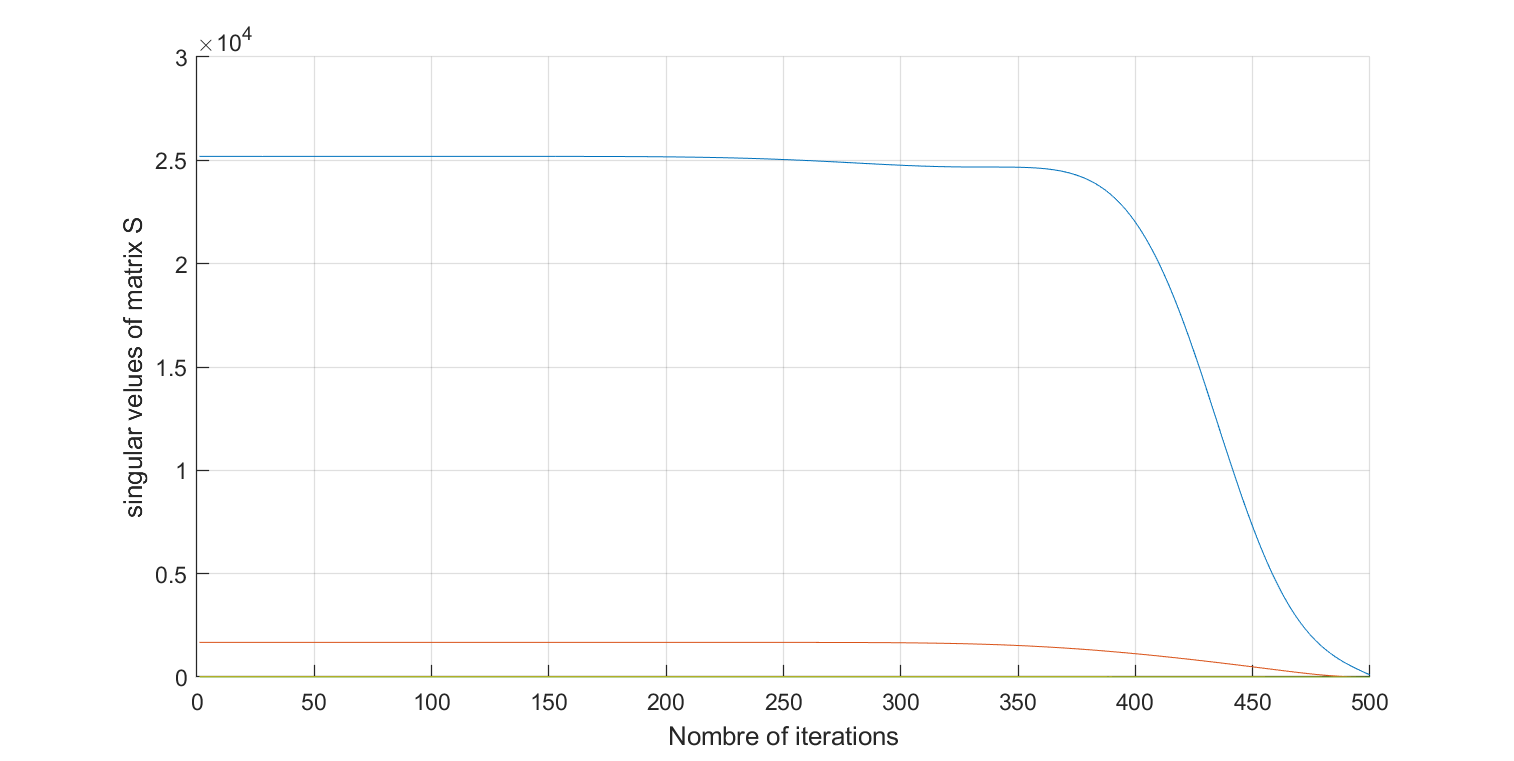
\includegraphics[width = 0.7\linewidth]{Latex report/image/ex2/svds.png}
    \caption{Evolution of singular values of S while solving the Riccati equation}
    \label{fig:svds}
\end{figure}




\subsection{Report the explicit value of the observation close loop poles, and the observer gain resulting
from it.}
The poles of the observer were designed to be 99.9\% of the poles of the closed loop dynamics and the following values have been found (3 significant digits) :

\begin{equation}
    \text{Observer poles :}
    \left[\begin{array}{c}
         0.999\\
         0.987\\
         0.0154\\
         0.985 + 0.0137i\\
         0.985 - 0.0137i\\
    \end{array}
    \right]
\end{equation}

Then by placing the poles of the observer, one may find the following observer gain :

\begin{equation}
    L = 
    \left[ {\begin{array}{ccccc}
        0.9845 &0      &0.01   &0         \\
        0      &0.0299 &0      &0         \\
        0      &0.0083 &0      &0.0008    \\
        0      &0      &0.0032 &0         \\
        0      &0      &0      &-0.0478   \\
    \end{array} } \right] 
\end{equation}

As a reminder, the Observer initial state has been set to zero. This will hold for every simulation.

\subsection{Provide a screen shot of your final Simulink scheme and the submodules you had to complete.}

\begin{figure}[H]
    \centering
    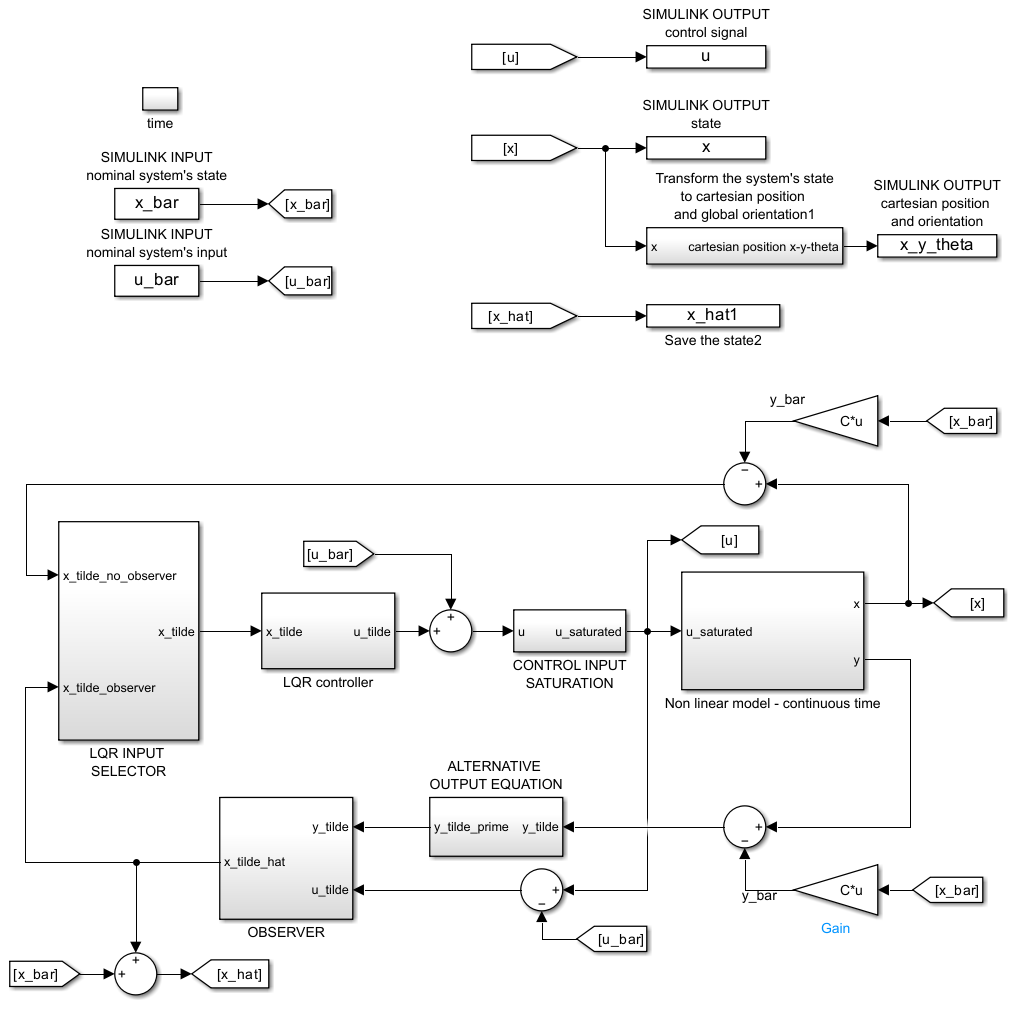
\includegraphics[width = 0.8\linewidth]{Latex report/image/ex2Simulink.png}
    \caption{Simulink diagram of exercise 2}
    \label{fig:ex2Simulink}
\end{figure}


\begin{figure}[H]
    \centering
         \begin{subfigure}[b]{0.8\textwidth}
         \centering
         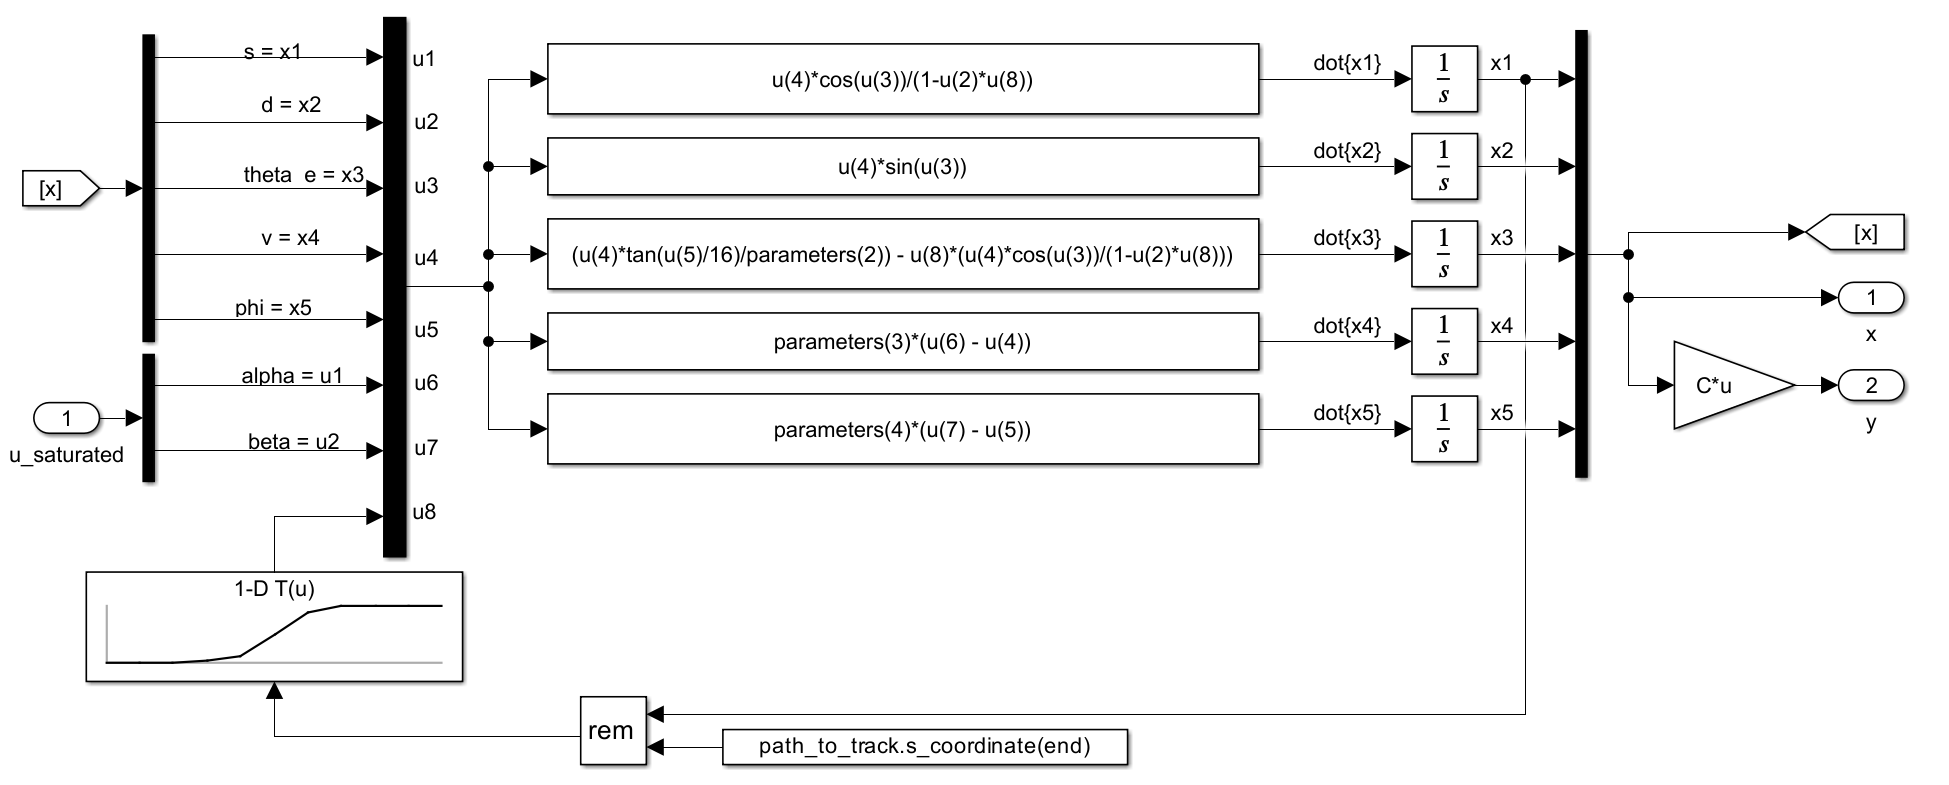
\includegraphics[width=\textwidth]{Latex report/image/nonLinModelContinousTimeEx2.png}
         \caption{Non linear model in continuous time implementation}
         \label{fig:nonLinSimulinkex2}
     \end{subfigure}
     \begin{subfigure}[b]{0.45\textwidth}
         \centering
         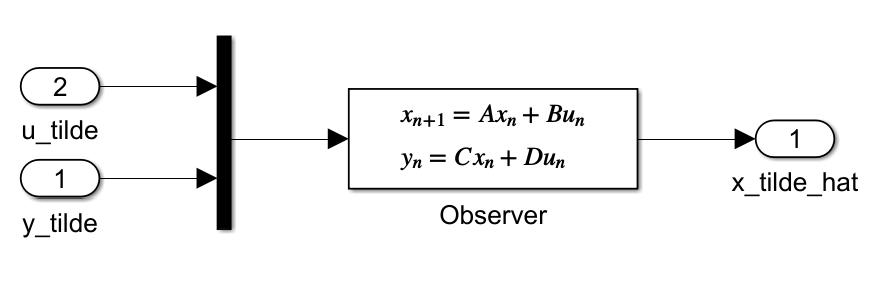
\includegraphics[width=\textwidth]{Latex report/image/ex2Observer.png}
         \caption{Observer implementation}
         \label{fig:ObsSim}
     \end{subfigure}
     \begin{subfigure}[b]{0.45\textwidth}
         \centering
         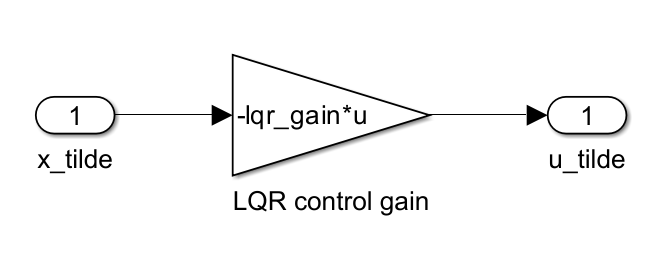
\includegraphics[width=\textwidth]{Latex report/image/Ex2LQR.png}
         \caption{LQR implementation}
         \label{fig:lqrSim}
     \end{subfigure}
     \begin{subfigure}[b]{0.45\textwidth}
         \centering
         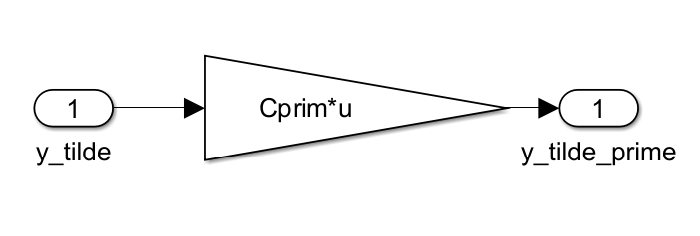
\includegraphics[width=\textwidth]{Latex report/image/ex2altEq.png}
         \caption{Alternative equation implementation}
         \label{fig:altEqSim}
     \end{subfigure}
     \begin{subfigure}[b]{0.45\textwidth}
         \centering
         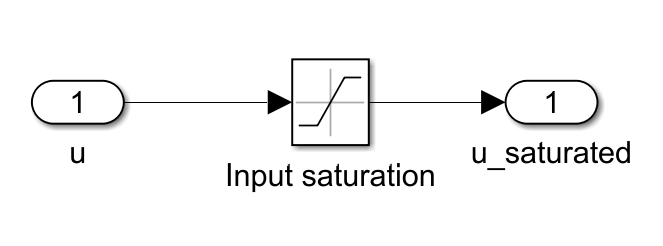
\includegraphics[width=\textwidth]{Latex report/image/ex2Saturation.png}
         \caption{Input saturation implementation}
         \label{fig:simSat}
     \end{subfigure}
    \caption{Implementation of the required block in simulink for exercise 2}
    \label{fig:simImplEx2}
\end{figure}

\subsection{Report the simulation results for the proposed values.}
The simulation with the proposed values is very satisfactory, the path is followed almost perfectly, with very little visible errors, in both cases : state measurement or observed state. In the estimation of the $x_3$ state, there are a tiny bit of irregularities, with the observer, which then leads to some error in control, especially in the heading error. This make sens and was awaited since, its the state variable with can't measure and have to estimate it. However, this could be corrected with a little bit of tuning, but it is not a problem for the overall control, since the vehicle still stay nicely on the track. We can see that the speed is almost constant (less than 1\% variation), so the vehicle is on time on the path, which tends to indicate that there is very little error in the other variables.

\begin{figure}[H]
    \centering
     \begin{subfigure}[b]{0.47\textwidth}
         \centering
         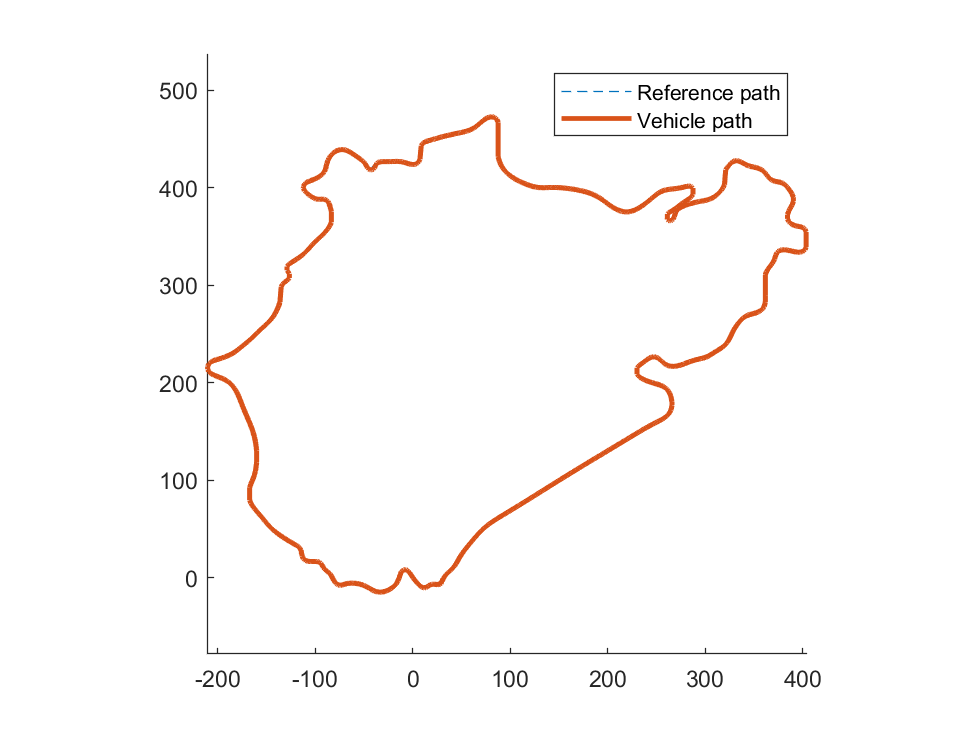
\includegraphics[width=\textwidth]{Latex report/image/ex2/trajectory1.png}
         \caption{Trajectory with state measurement}
         \label{fig:traj21}
     \end{subfigure}
     \begin{subfigure}[b]{0.47\textwidth}
         \centering
         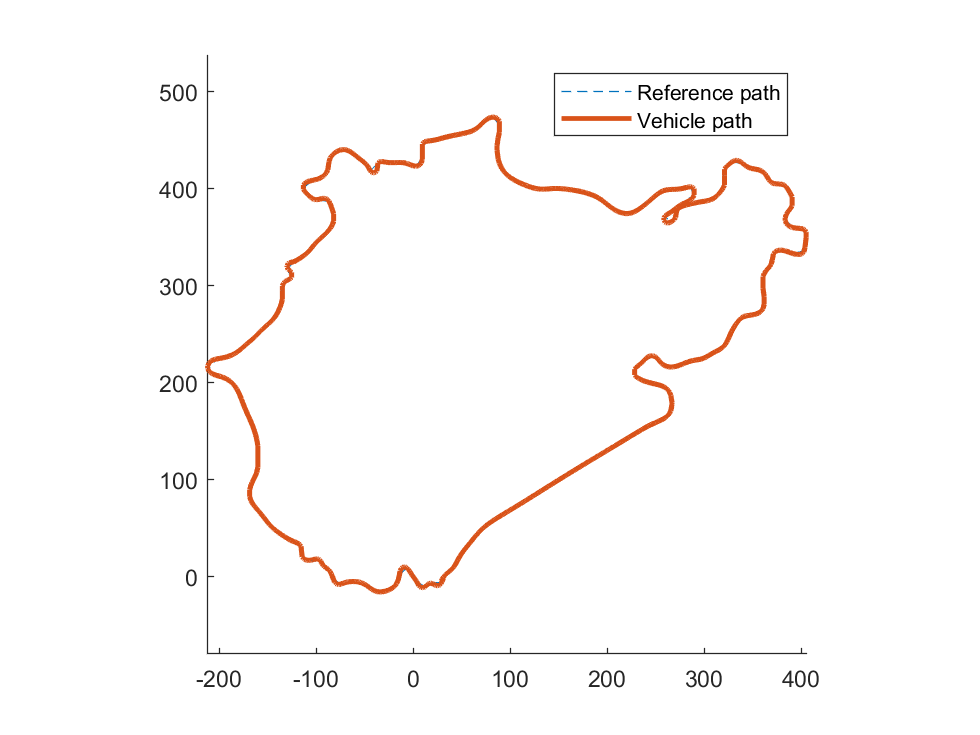
\includegraphics[width=\textwidth]{Latex report/image/ex2/trajectory.png}
         \caption{Trajectory with Observed state}
         \label{fig:traj22}
     \end{subfigure}
     \begin{subfigure}[b]{0.47\textwidth}
         \centering
         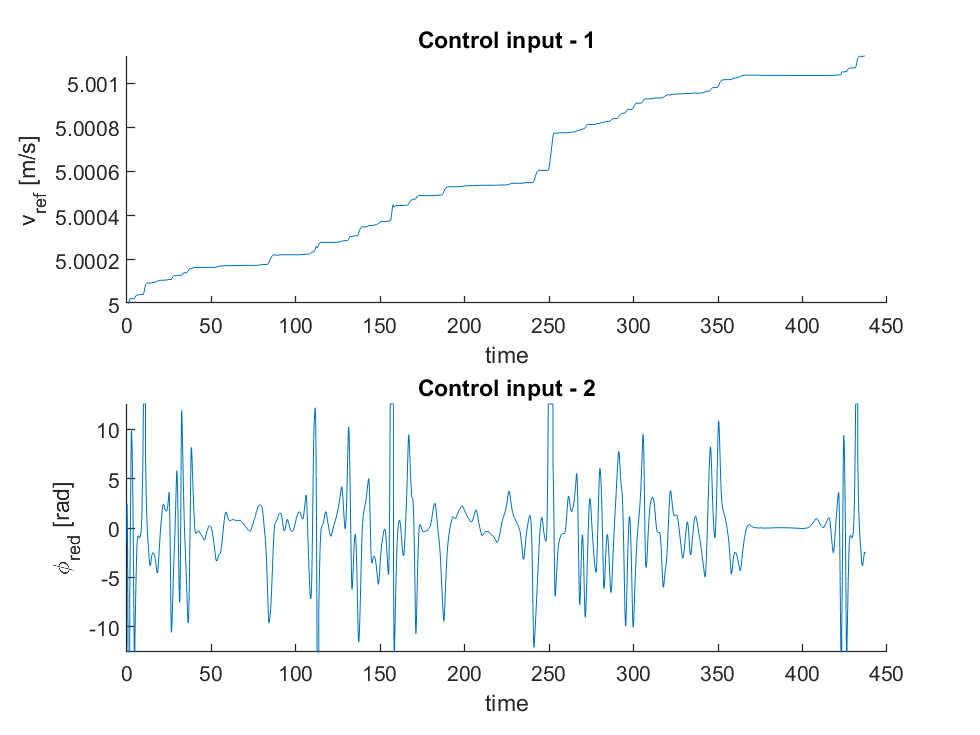
\includegraphics[width=\textwidth]{Latex report/image/ex2/input1.png}
         \caption{Control input with state measurement}
         \label{fig:input21}
     \end{subfigure}
     \begin{subfigure}[b]{0.47\textwidth}
         \centering
         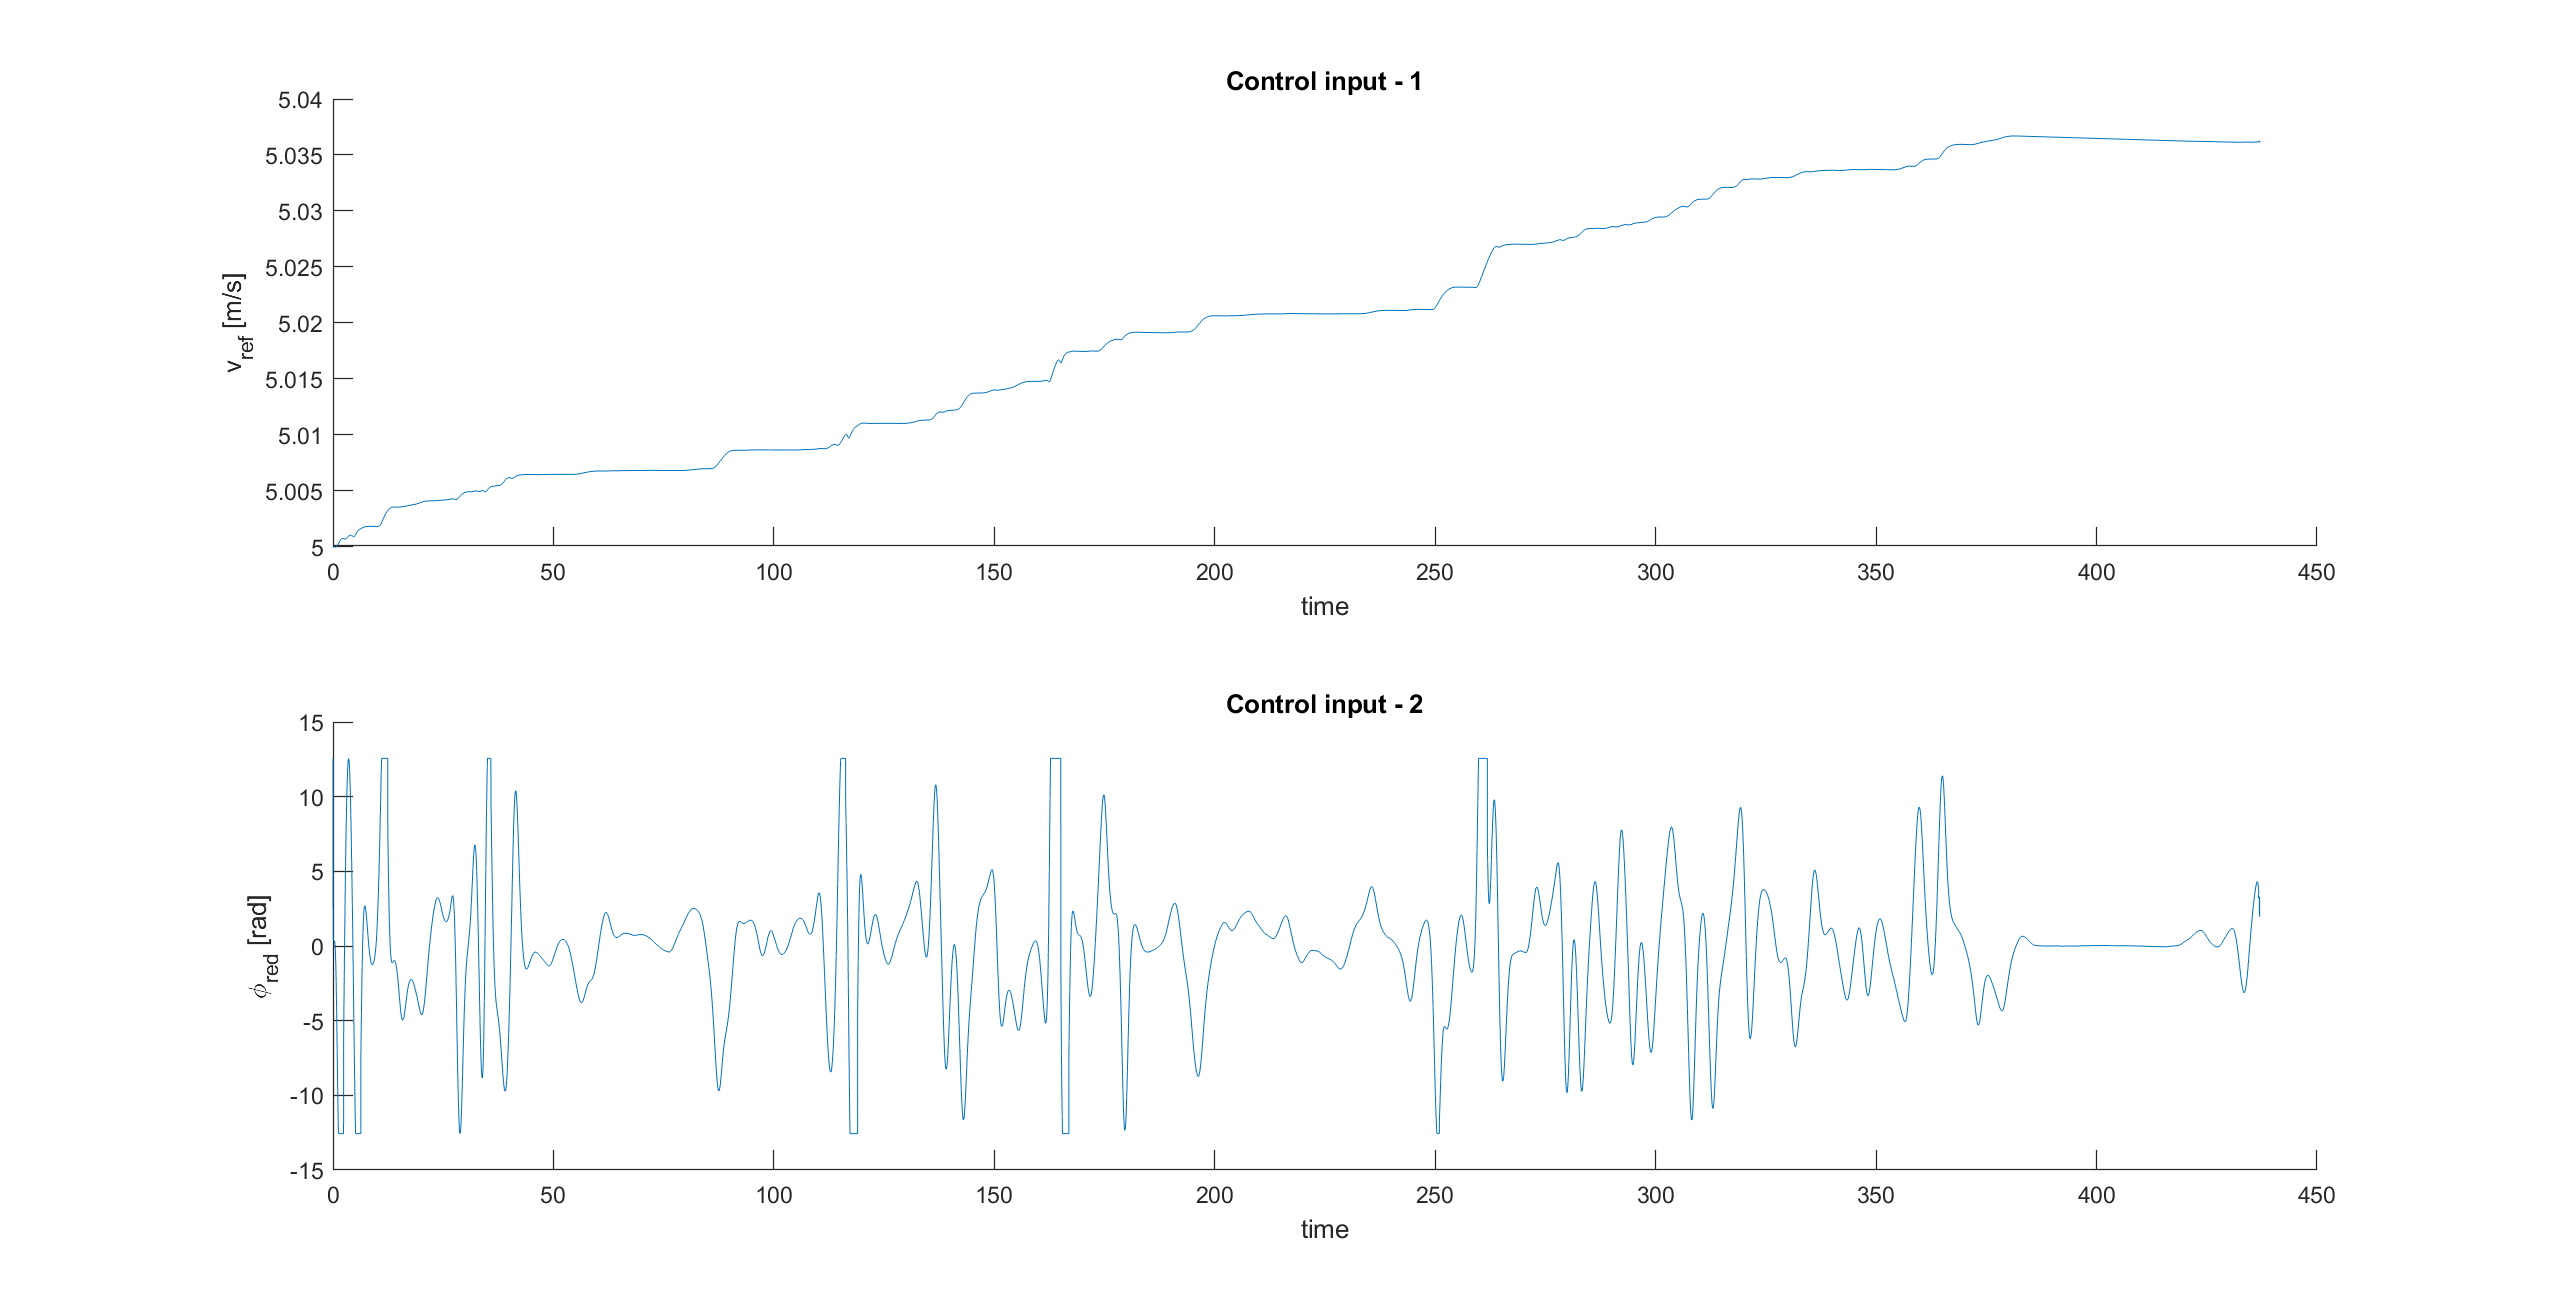
\includegraphics[width=\textwidth]{Latex report/image/ex2/input.png}
         \caption{Control input with Observed state}
         \label{fig:input22}
     \end{subfigure}
     \begin{subfigure}[b]{0.95\textwidth}
         \centering
         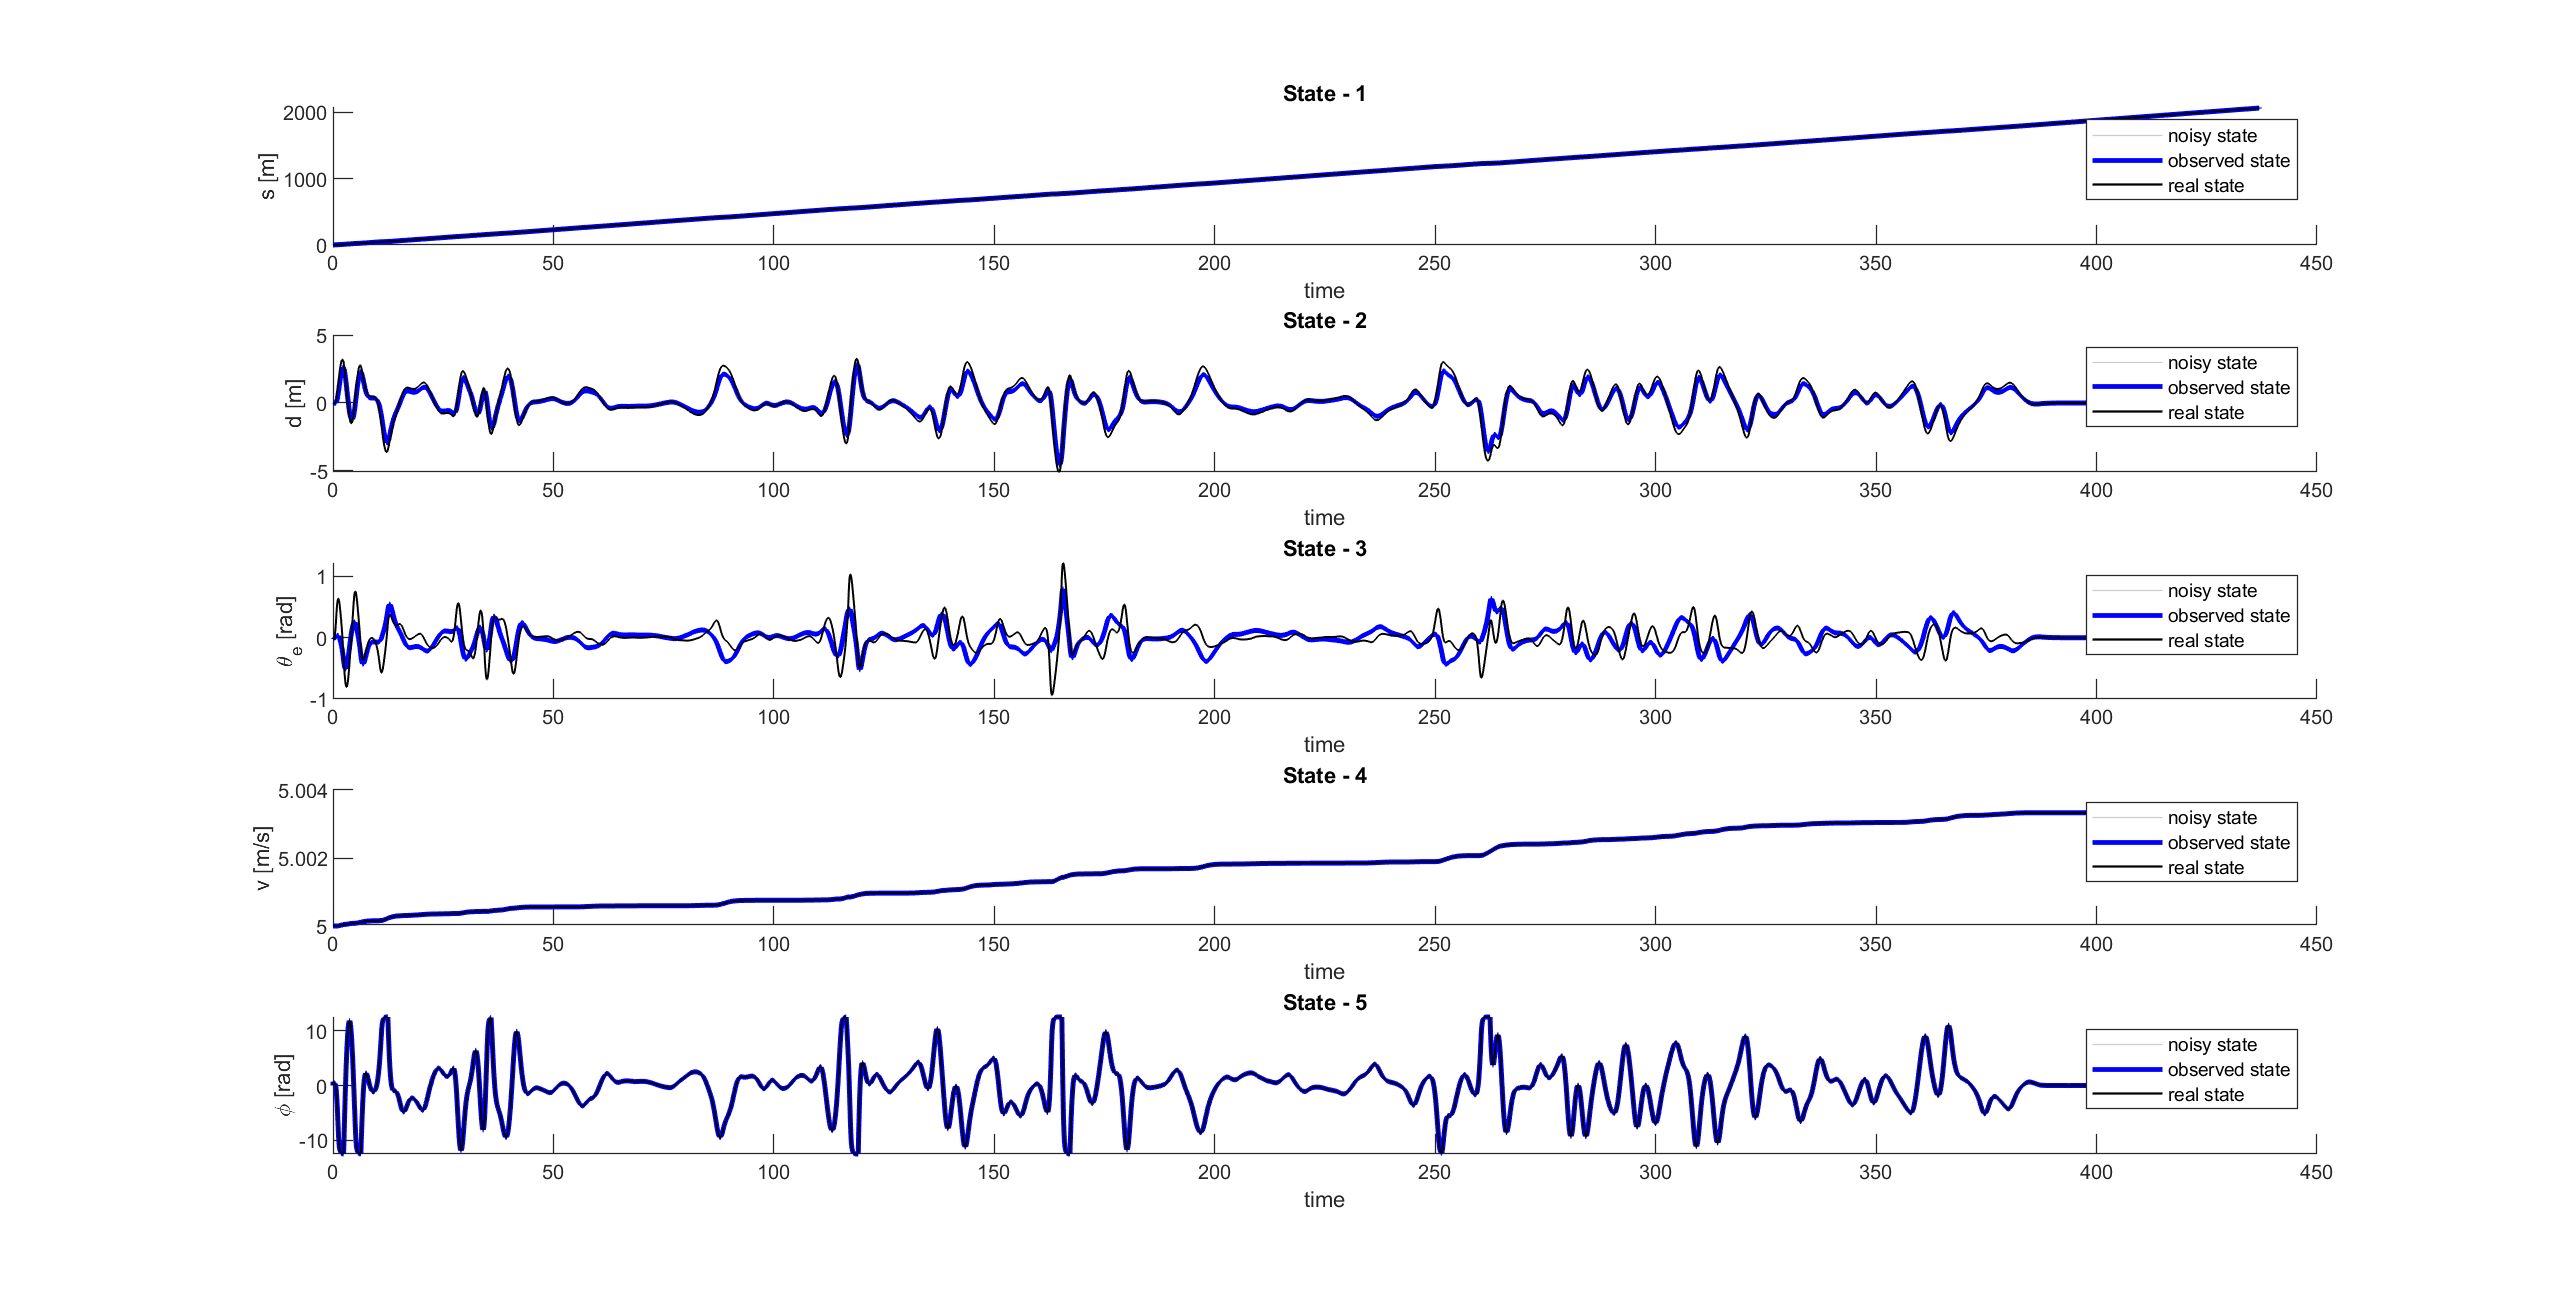
\includegraphics[width=\textwidth]{Latex report/image/ex2/obs.png}
         \caption{Comparison of the states between state measurement and Observed state}
         \label{fig:Obs}
     \end{subfigure}
    \caption{Simulation of the LQR regulator with and without an observer}
    \label{fig:sim}
\end{figure}

\subsection{The proposed value of Q1 intends to assign very little importance to the error deriving from x1. Could you explain why doing this might make sense?}

First, $x_1$ represents $s$, the distance travelled along the path, which is a function of all the other variables (indirectly for $x_5$), whereas none of the other variables is a function of $x_1$. This means that if there is no error (or accumulated error) in the other variables, there is none in $x_1$ either. Efficiently controlling $x_2$, $x_3$, $x_4$ and $x_5$ also controls $x_1$. Moreover, the error in $x_1$ represents the time advance or delay that the vehicle has on the path, which will result in accelerating or decelerating the vehicle (term $K_{LQR,11}$). One can imagine that if the vehicle accelerates greatly, it becomes increasingly difficult or impossible to control the vehicle. To have a robust controller, it is therefore natural to limit the weight of the error in $x_1$.



\subsection{Propose a different pair Q1 and Q2 such that heading deviation error is highly penalized compared to the other states and report simulation results where the impact of doing so can be clearly observed.}
The new proposed $Q_1$ and $Q_2$ are :
\begin{equation}
    Q_1 = 
    \left[ {\begin{array}{ccccc}
        1e-5 &0   &0   &0   &0     \\
        0    &0.5 &0   &0   &0     \\
        0    &0   &50  &0   &0     \\
        0    &0   &0   &0.5 &0     \\
        0    &0   &0   &0   &0.5   \\
    \end{array} } \right]    
    ,\quad
    Q_2 =
    \left[ {\begin{array}{cc}
        1 &0\\
        0 &2e-5\\
    \end{array} } \right]
\end{equation}

The value of the LQR gain obtained by solving the Riccati equation are :
\begin{equation}
    K_{LQR} = 
    \left[ {\begin{array}{ccccc}
         3.99e-4 &0       &0       &0.2237 &0      \\
         0         &20.067 &304.03 &0      &19.308 \\
    \end{array}}\right]
\end{equation}
This time, the control problem is more challenging, thus a simpler reference path has been chosen. Even though, the vehicle is no longer tracked on the path and control is completely lost. This is partly due to the fact that the control of $x_3$ is aggressive (large weight on $x_3$ in $Q_1$) while this variable is not measured but estimated. There is a discrepancy between the real and estimated state of $x_3$. The observer is too slow to correct this error, which then induce more error in the tracking of the path until the control gets finally out of hand. Tuning of the observer dynamics is further needed to achieve control of the vehicle. Indeed, the observer dynamic is almost equal to the dynamic of the system, which is too slow to correct estimation error on $x_3$.

\begin{figure}[H]
    \centering
     \begin{subfigure}[b]{0.47\textwidth}
         \centering
         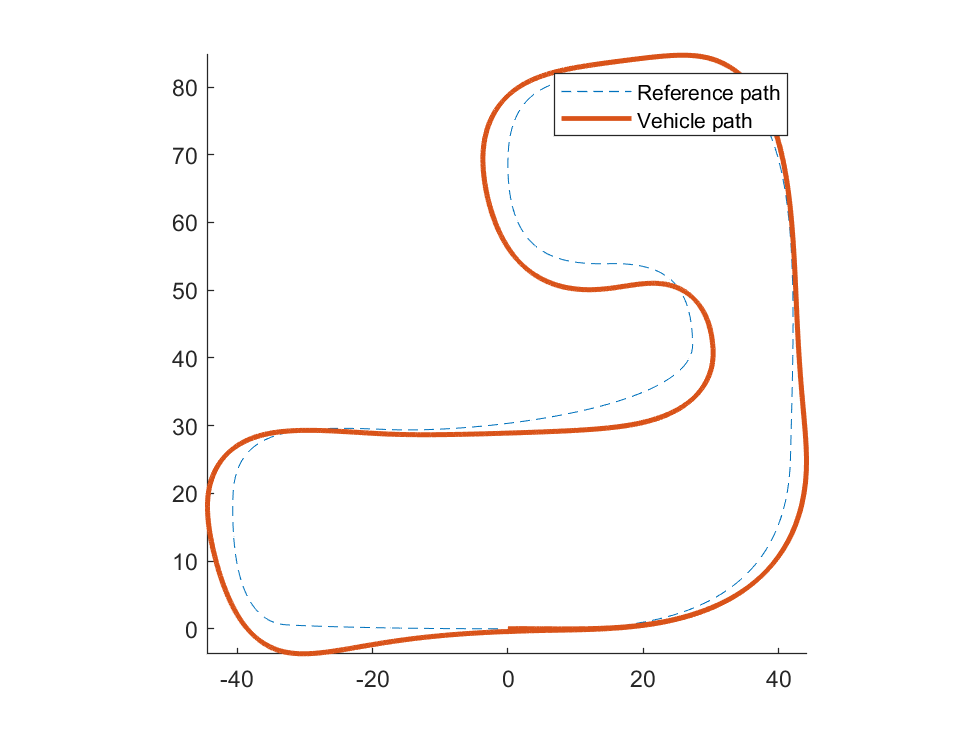
\includegraphics[width=\textwidth]{Latex report/image/ex2/trajectory12.png}
         \caption{Trajectory with state measurement}
         \label{fig:traj31}
     \end{subfigure}
     \begin{subfigure}[b]{0.47\textwidth}
         \centering
         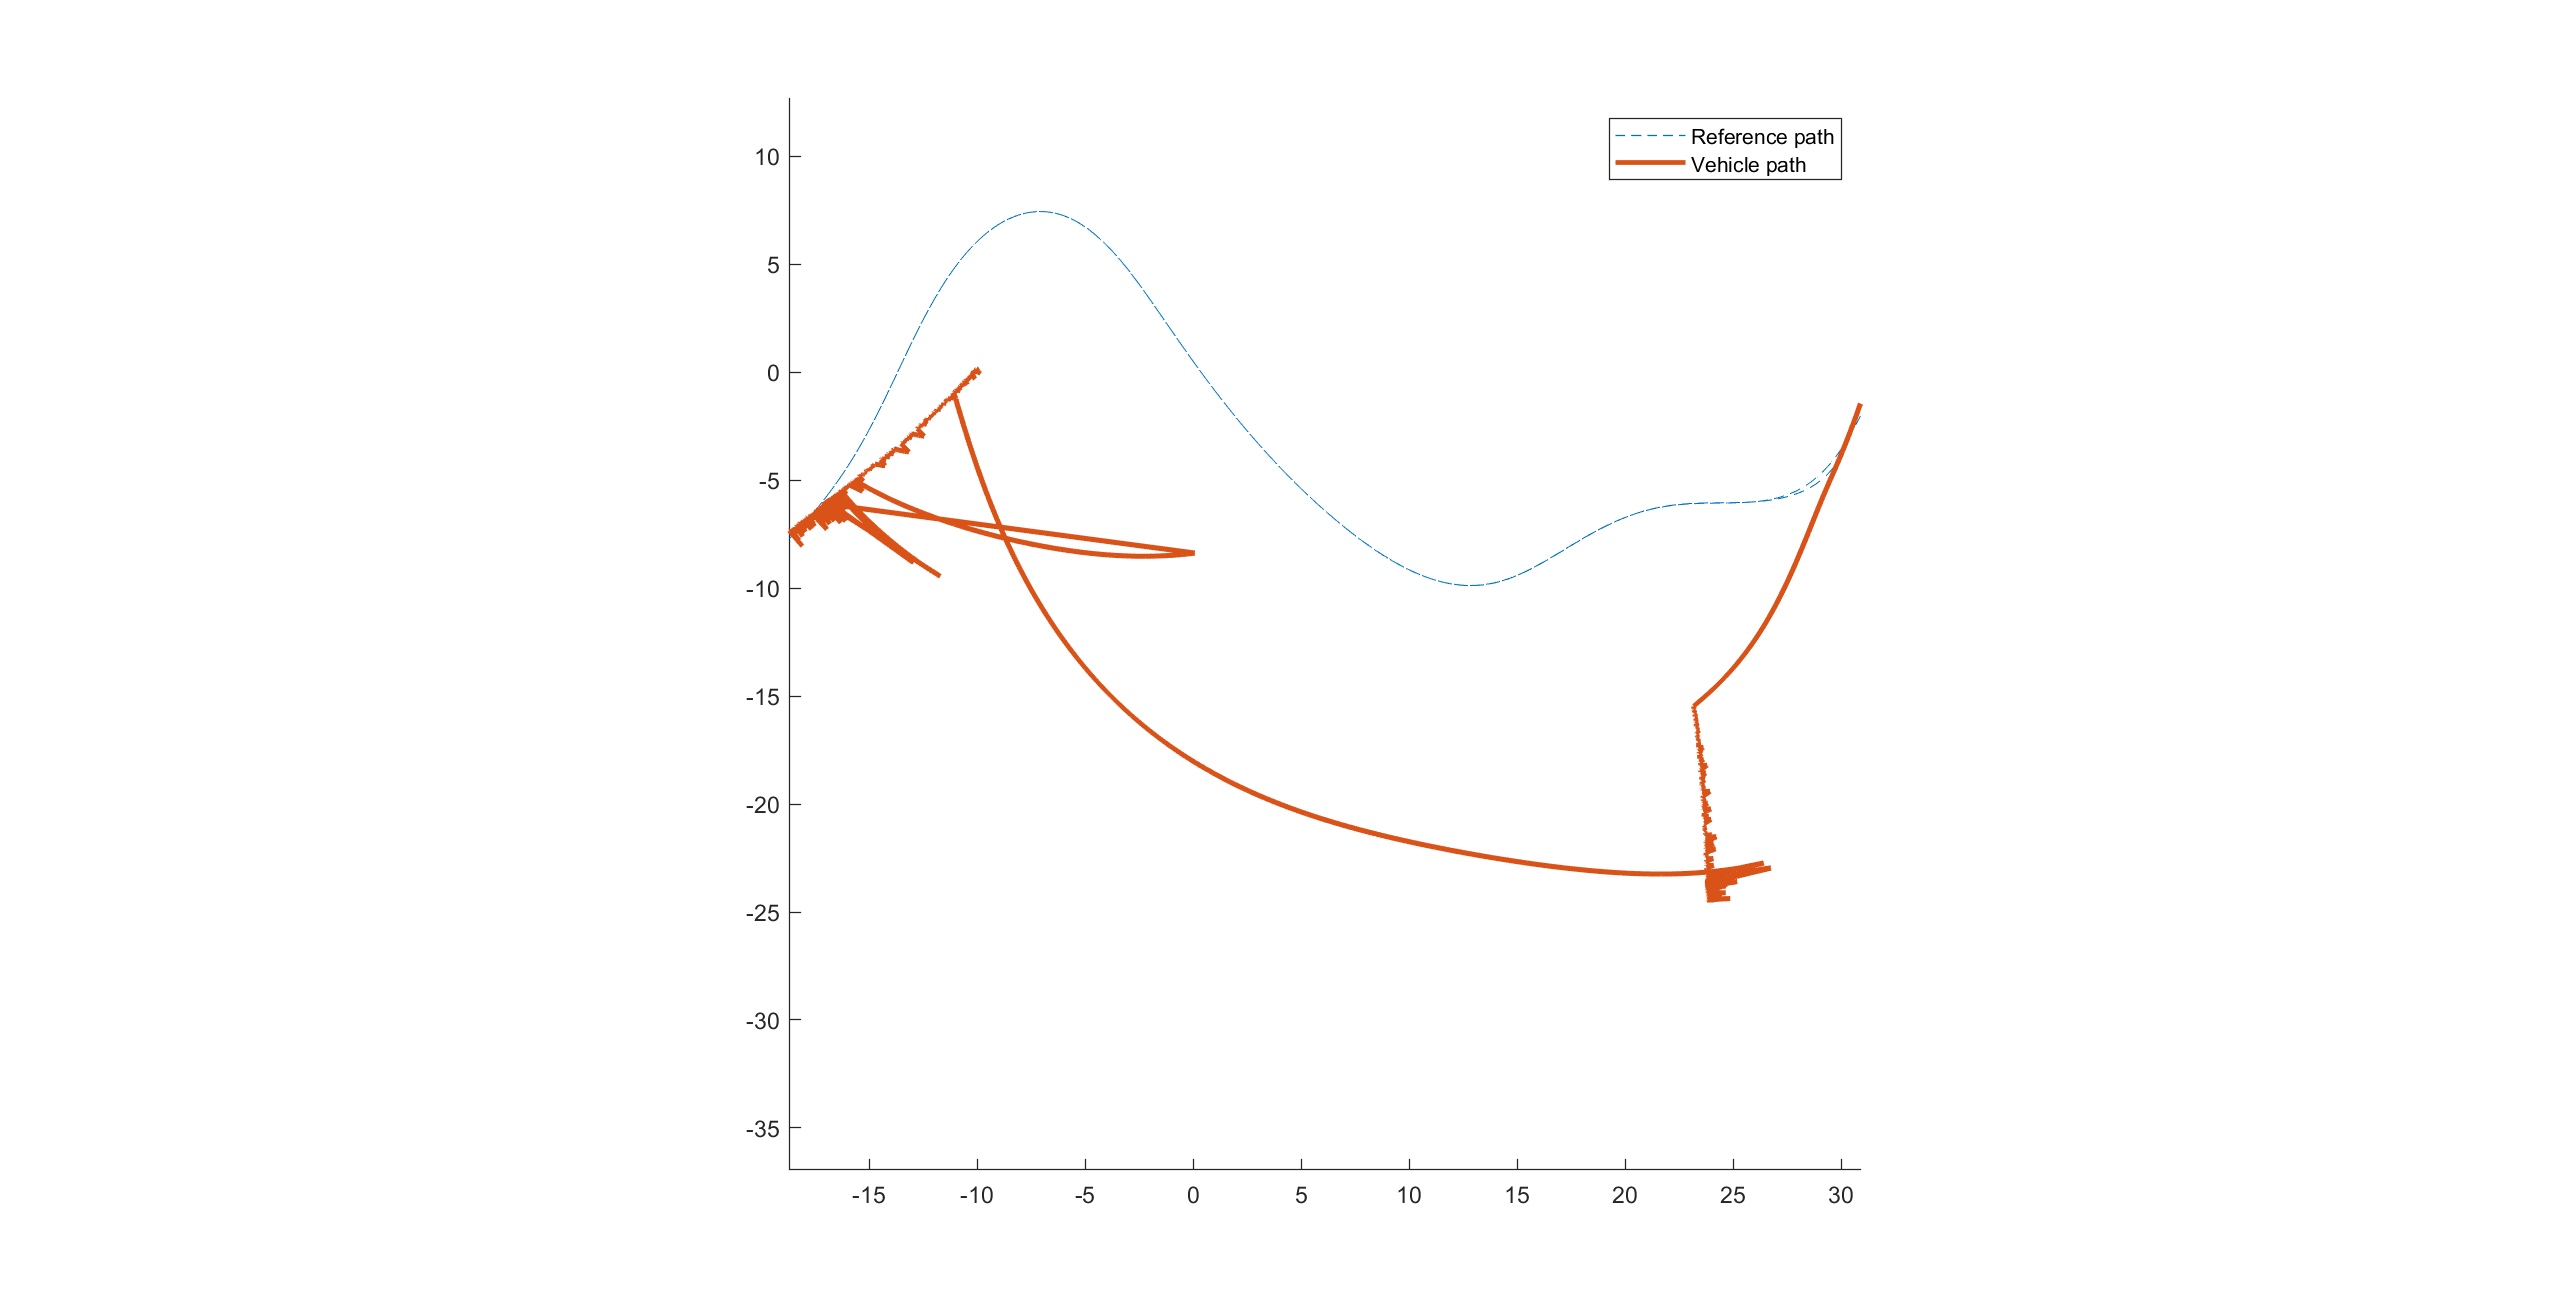
\includegraphics[width=\textwidth]{Latex report/image/ex2/trajectory2.png}
         \caption{Trajectory with Observed state}
         \label{fig:traj32}
     \end{subfigure}
     \begin{subfigure}[b]{0.47\textwidth}
         \centering
         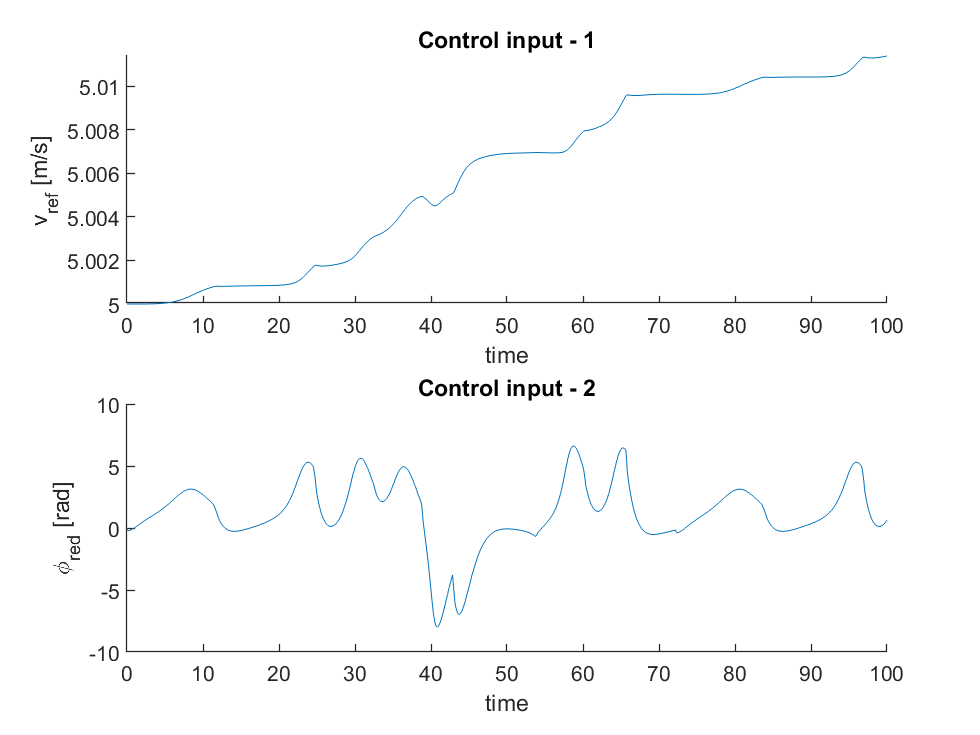
\includegraphics[width=\textwidth]{Latex report/image/ex2/input12.png}
         \caption{Control input with state measurement}
         \label{fig:input31}
     \end{subfigure}
     \begin{subfigure}[b]{0.47\textwidth}
         \centering
         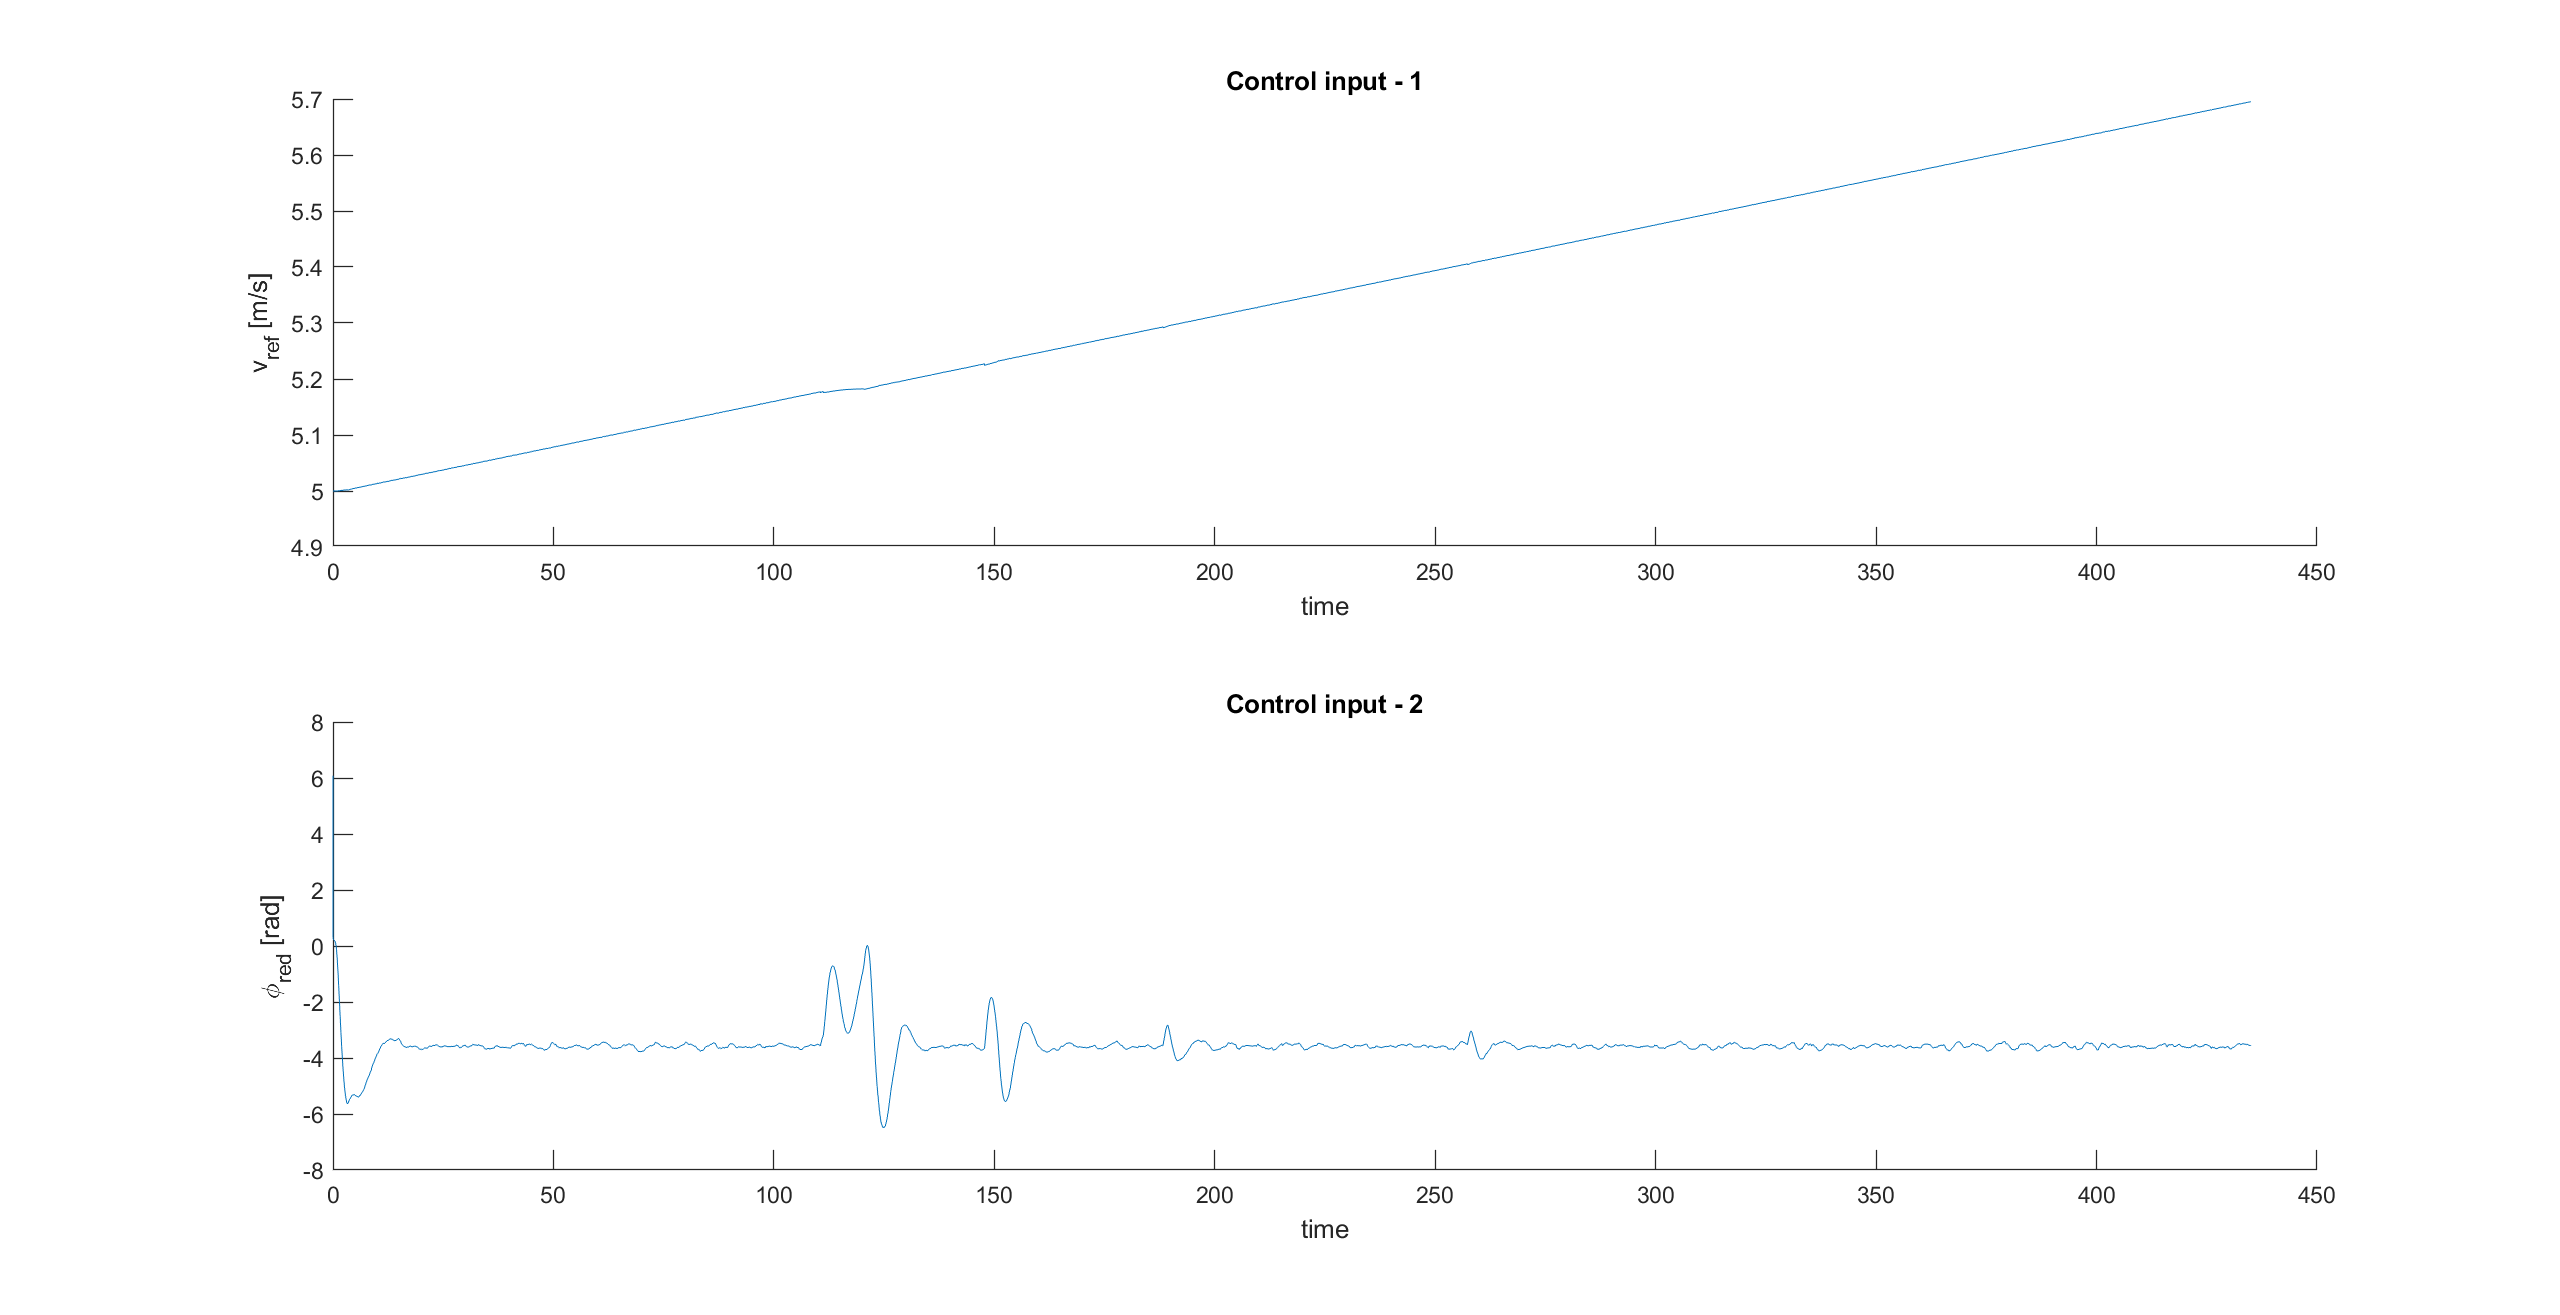
\includegraphics[width=\textwidth]{Latex report/image/ex2/input2.png}
         \caption{Control input with Observed state}
         \label{fig:input32}
     \end{subfigure}
     \begin{subfigure}[b]{0.95\textwidth}
         \centering
         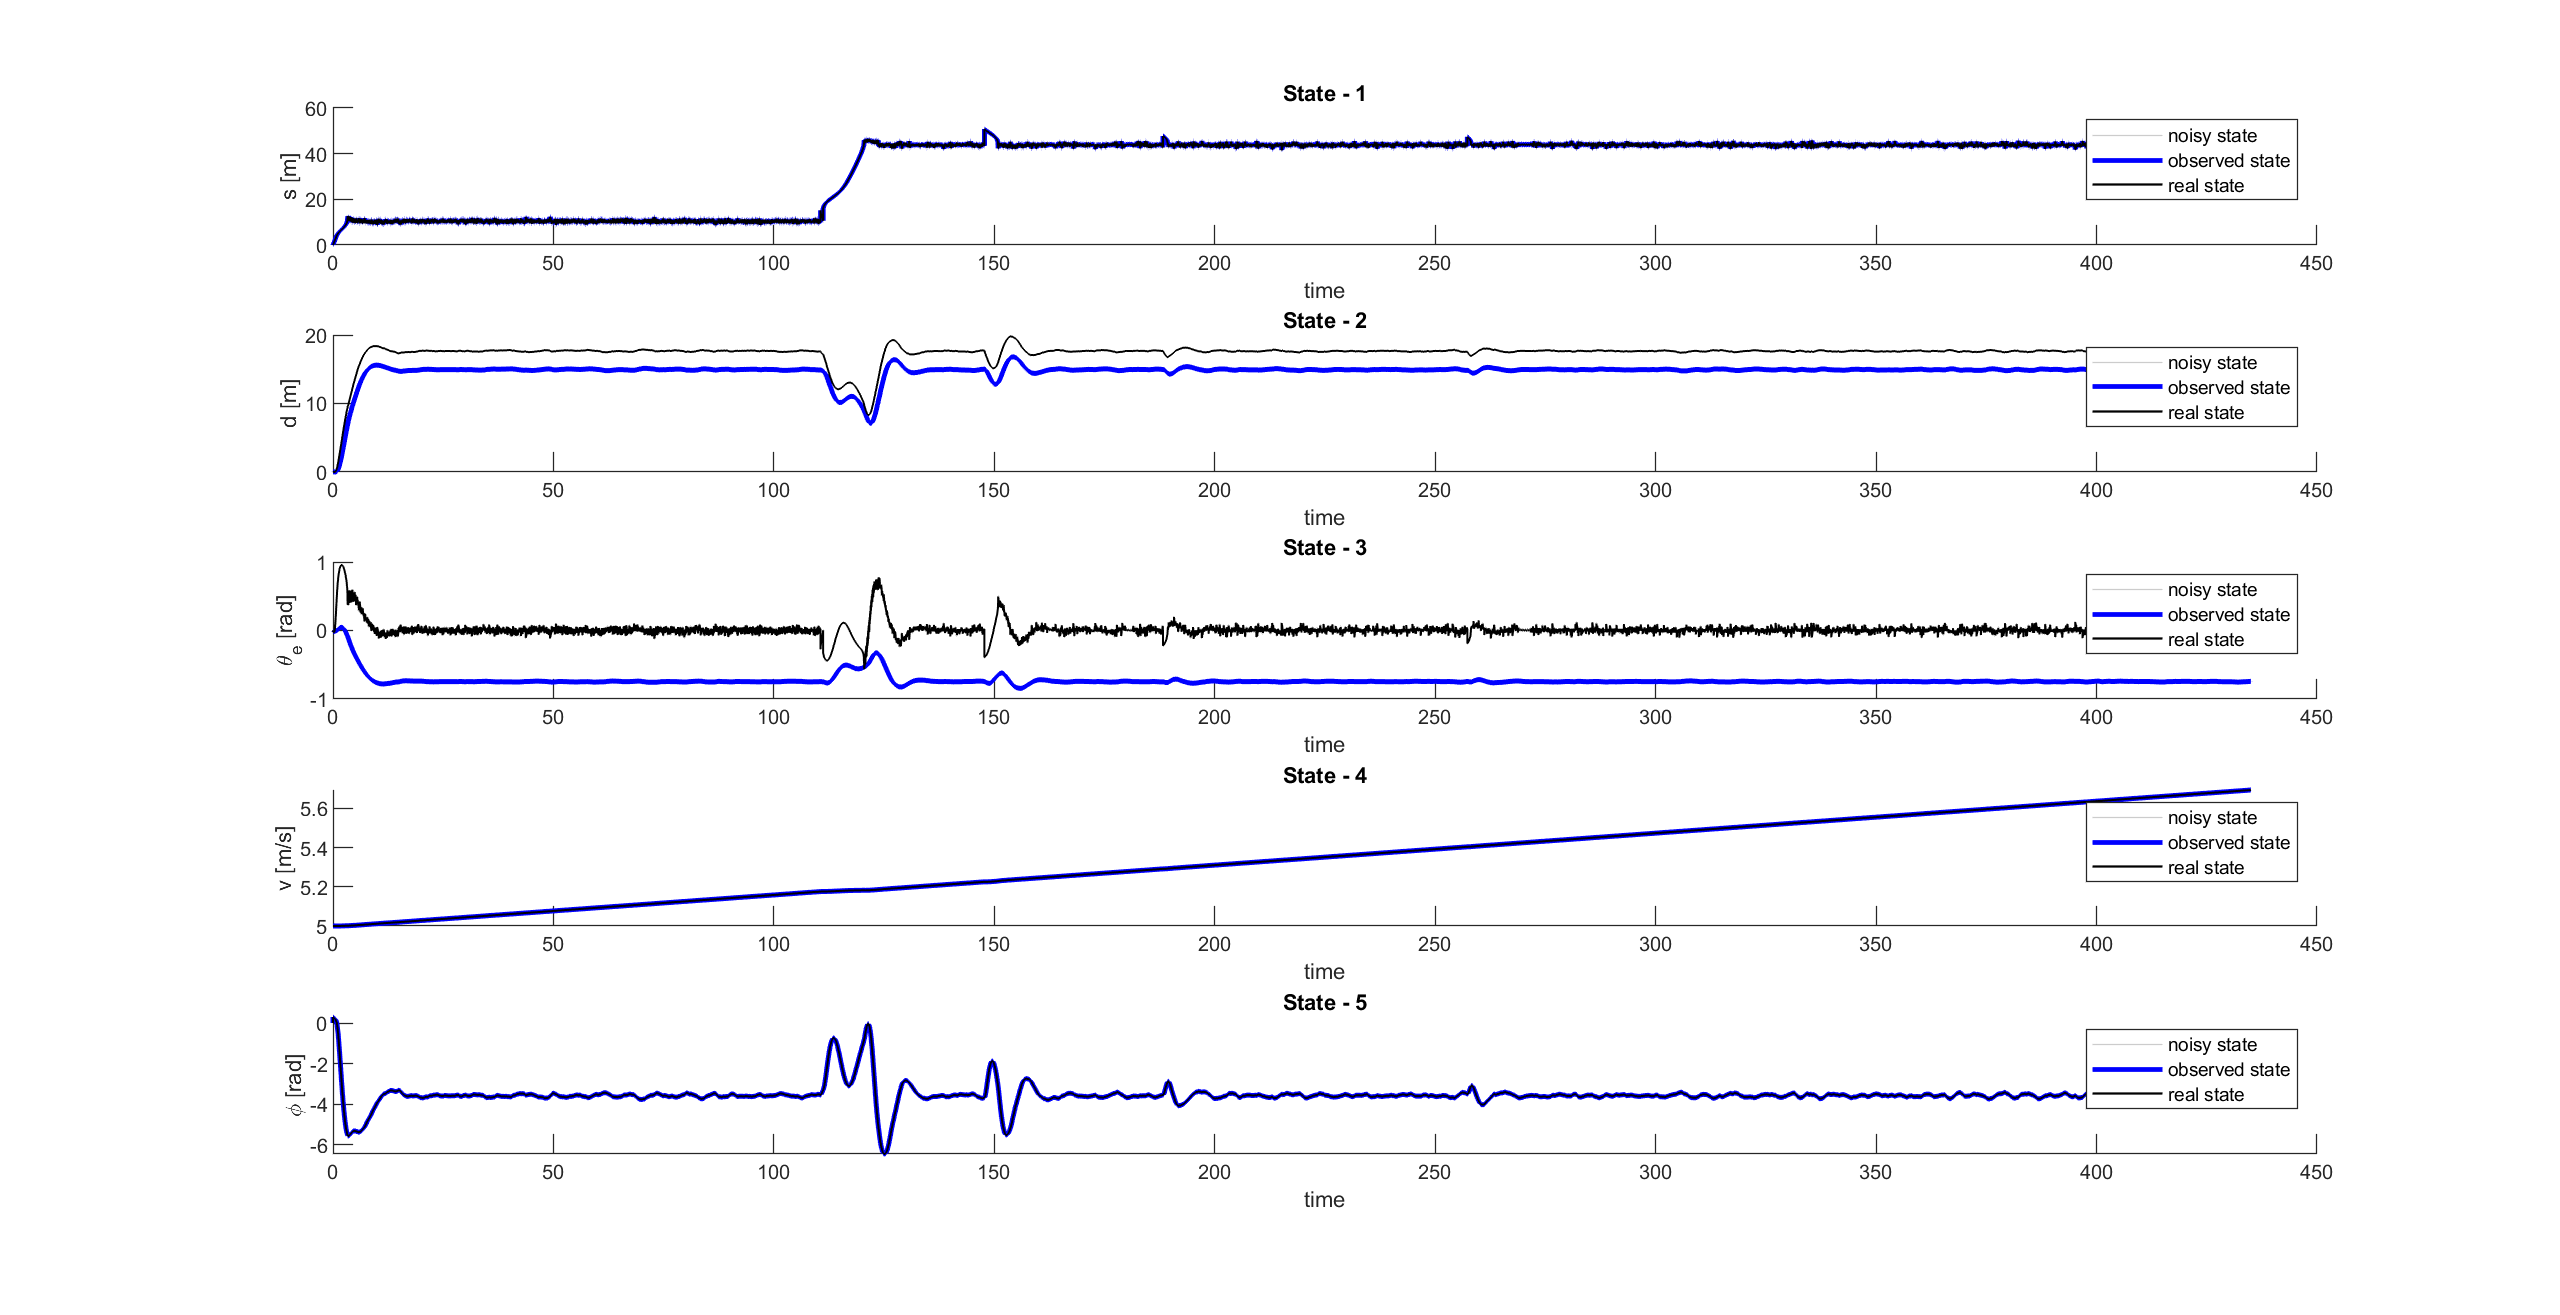
\includegraphics[width=\textwidth]{Latex report/image/ex2/obs2.png}
         \caption{Comparison of the states between state measurement and Observed state}
         \label{fig:Obs2}
     \end{subfigure}
    \caption{Simulation of the LQR regulator with an observer and new pole placement}
    \label{fig:sim2}
\end{figure}


\subsection{Is the proposed placement for the observation close loop poles appropriate? why? If not,propose a new set of poles to improve the observation performance.}

As mentioned above, the control of the vehicle with these new parameters failed because the observer was too slow to correct the error in the estimation of between the states and so the control got carried away and could not catch up. One solution is to impose a more aggressive dynamic on the estimation of the states on the observer. In the results below, the poles of the observer have been chosen to be 1\% of the poles of the system dynamics.
\begin{equation}
    \text{Observer poles :}
    \left[\begin{array}{c}
         0.01\\
         0.00988\\
         0.000154\\
         0.00994 + 205e-5i\\
         0.00994 - 205e-5i\\
    \end{array}\right]
\end{equation}

It turns out that with this new observer, the vehicle is again very well controlled and follows the reference path correctly. We can see that the estimated state has no error at all compared to the true state which was not the case with the two previous simulations, which suggest that the observer was correctly tune this time. Since, for this last simulation, its the observer's performances that are evaluated, only its results are presented for visibility purpose.

\begin{figure}[H]
    \centering
     \begin{subfigure}[b]{0.45\textwidth}
         \centering
         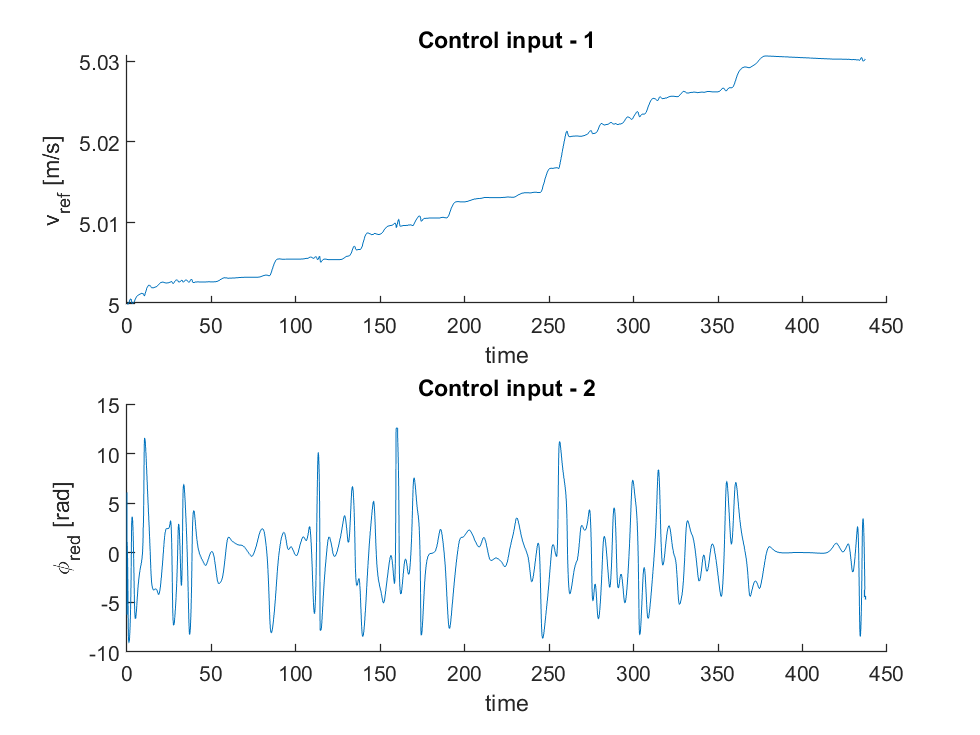
\includegraphics[width=\textwidth]{Latex report/image/ex2/inputNewpole.png}
         \caption{Control input}
         \label{fig:NPinput}
     \end{subfigure}
     \begin{subfigure}[b]{0.45\textwidth}
         \centering
         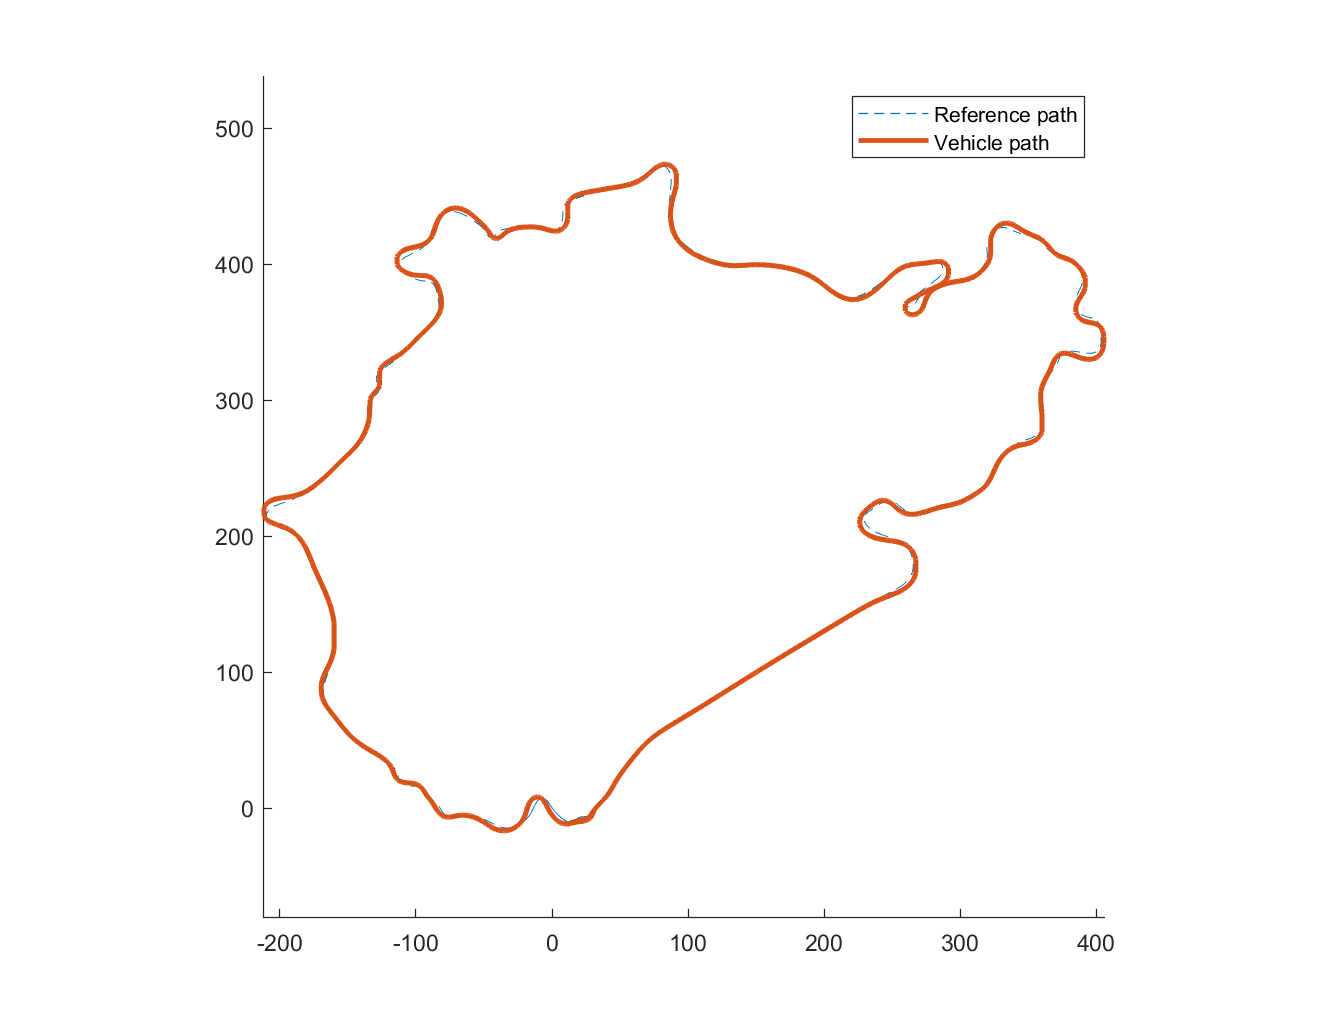
\includegraphics[width=\textwidth]{Latex report/image/ex2/trajectoryNewpole.png}
         \caption{Trajectory}
         \label{fig:NPtraj}
     \end{subfigure}
     \begin{subfigure}[b]{0.8\textwidth}
         \centering
         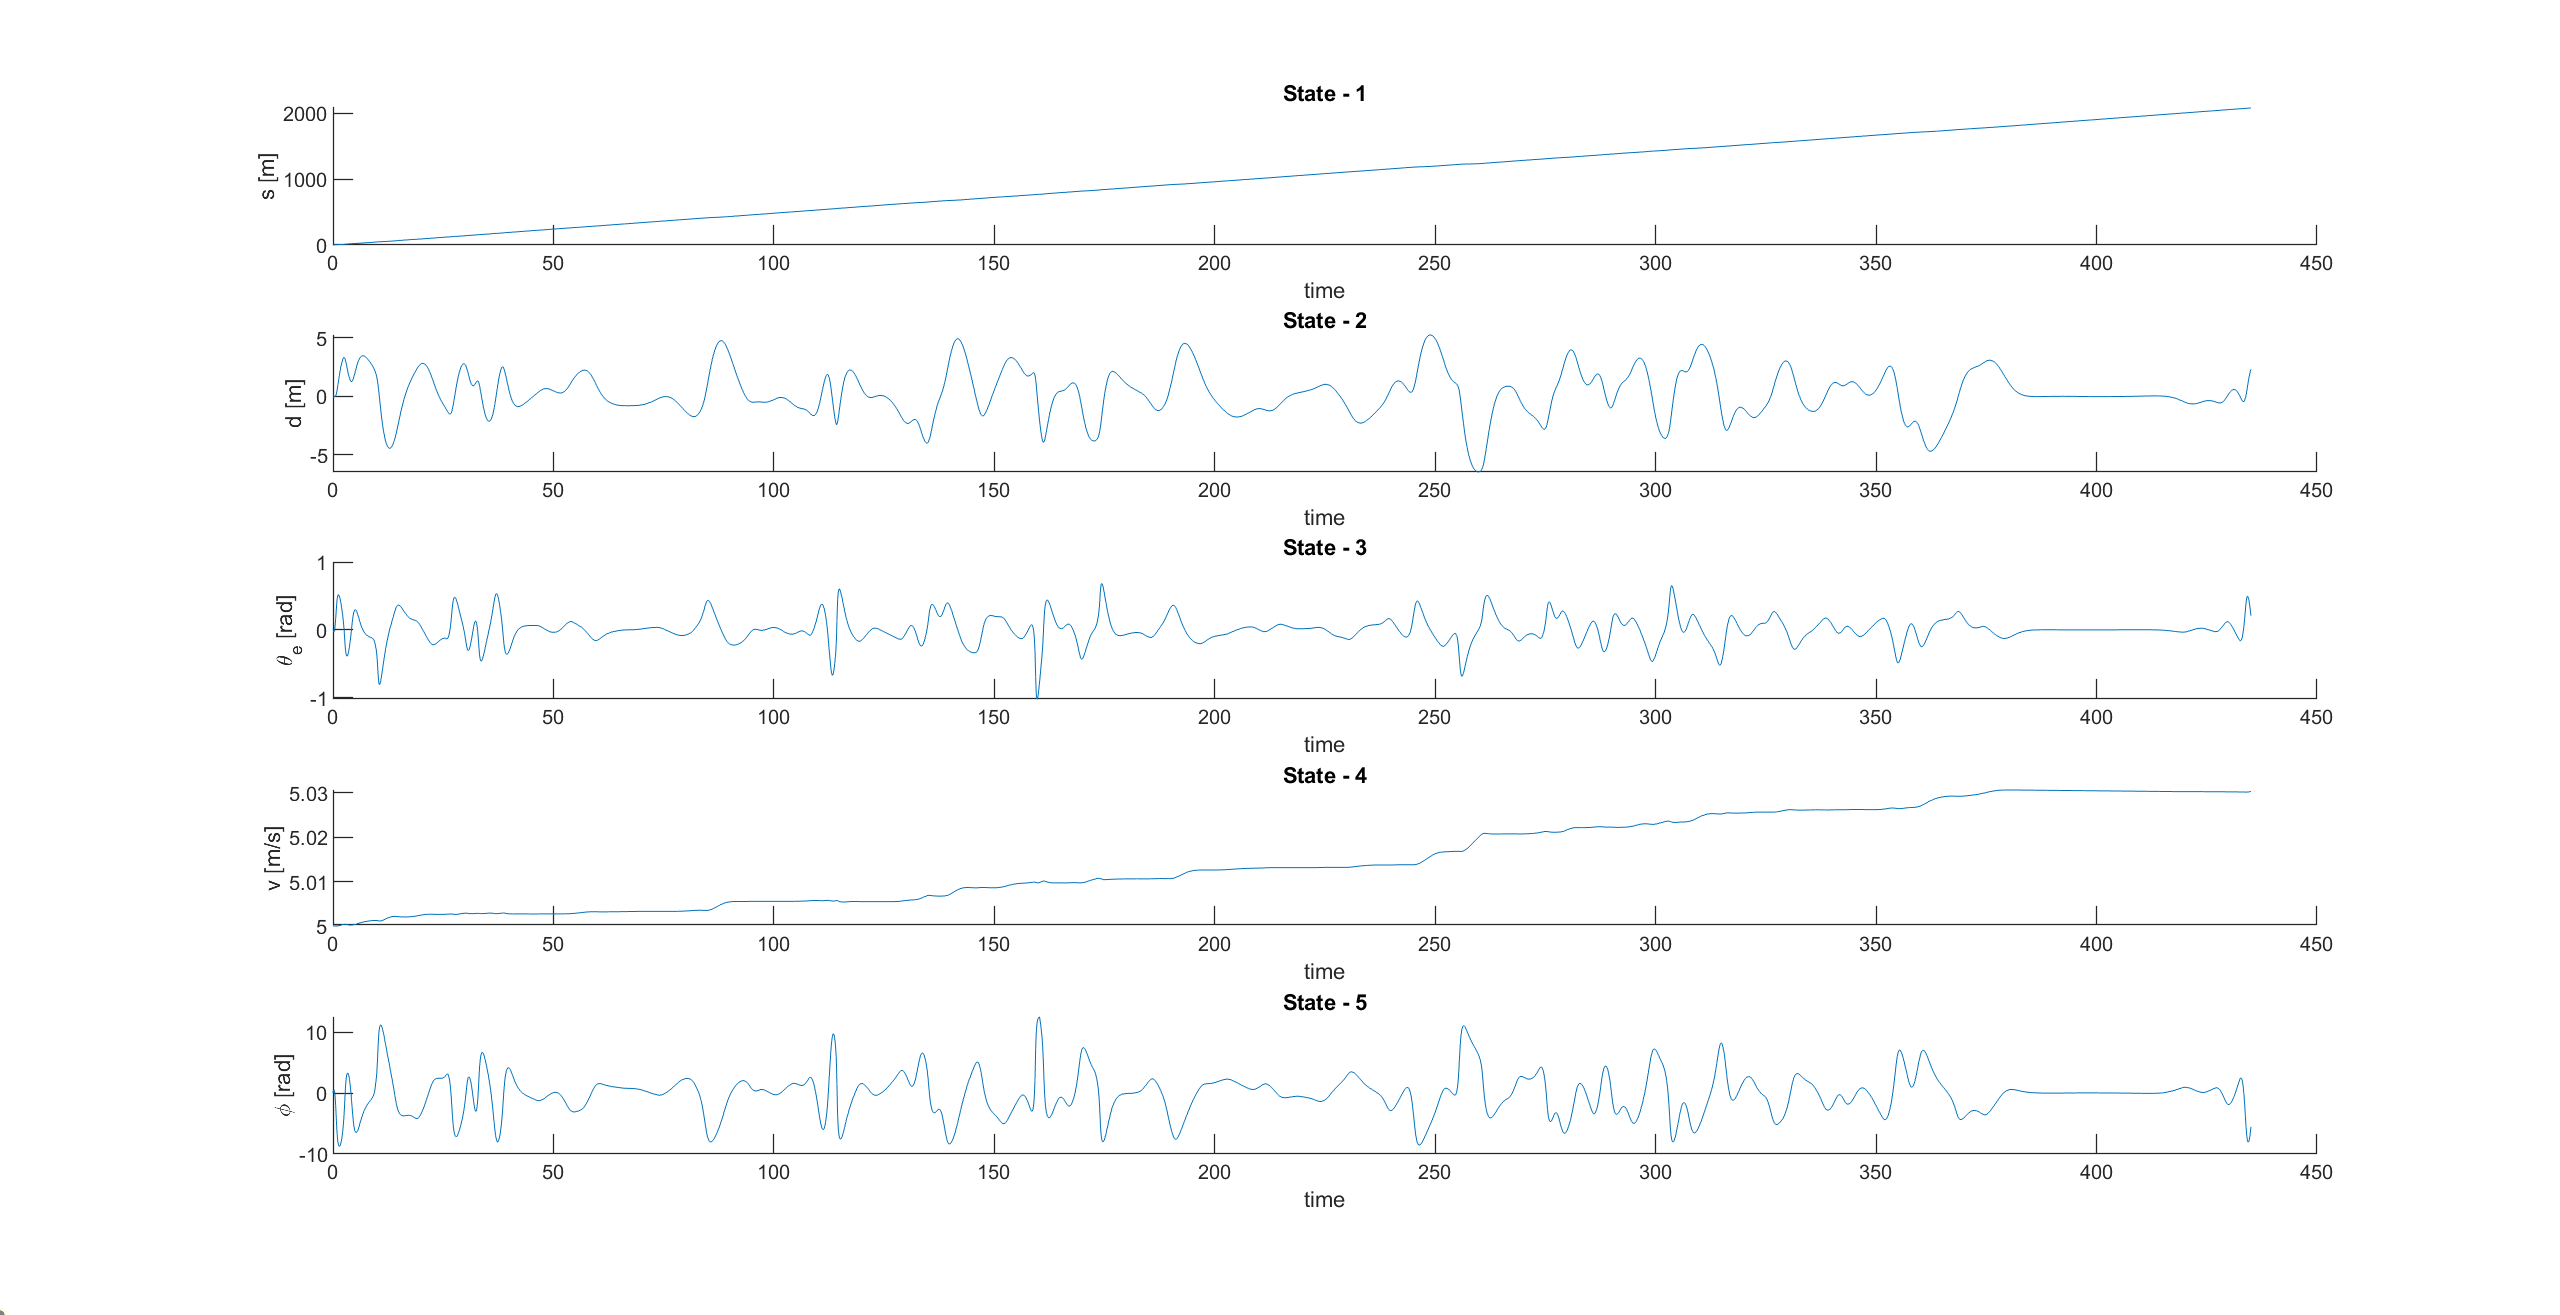
\includegraphics[width=\textwidth]{Latex report/image/ex2/stateNewpole.png}
         \caption{Observed state}
         \label{fig:NPState}
     \end{subfigure}
     \begin{subfigure}[b]{0.8\textwidth}
         \centering
         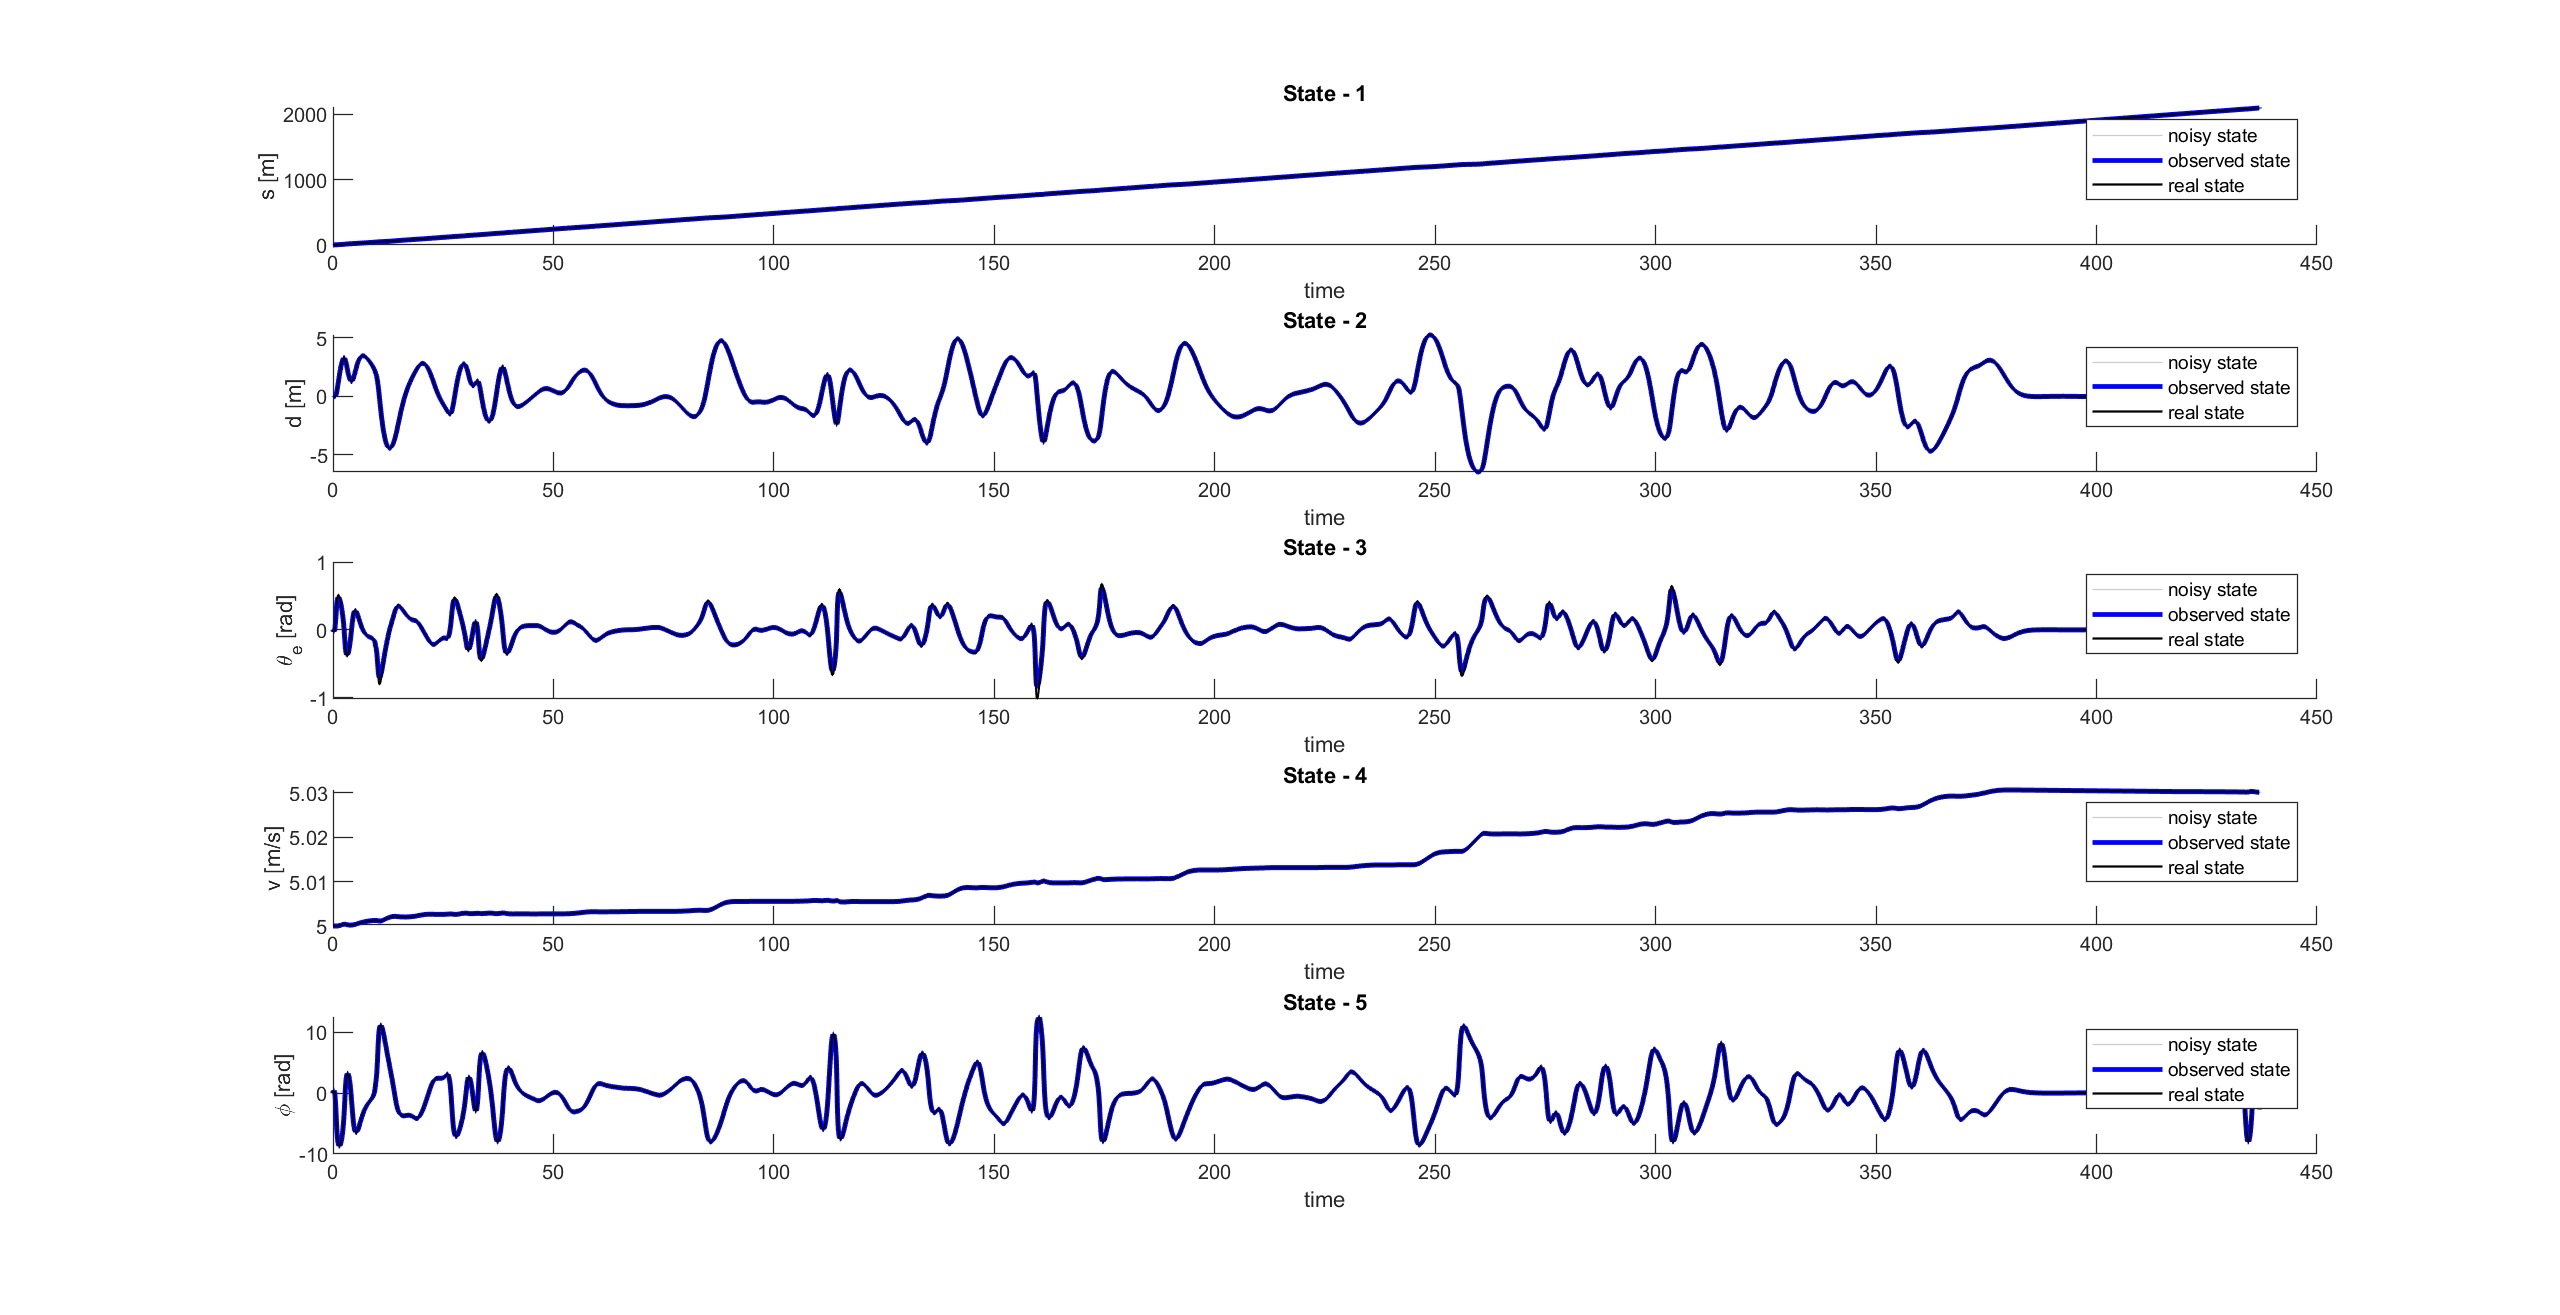
\includegraphics[width=\textwidth]{Latex report/image/ex2/obsNewpole.png}
         \caption{Comparison with state measurement}
         \label{fig:NPObs}
     \end{subfigure}
    \caption{Simulation of the LQR regulator with an observer and new pole placement}
    \label{fig:NP}
\end{figure}





\newpage
\printbibliography 

\end{document}
